\documentclass[12pt]{article}
	\usepackage{amsmath}
	\usepackage{amssymb}
	\usepackage{fancyhdr}
	\usepackage{float}
	\usepackage{graphicx}
	\usepackage{cite}
	\usepackage{mathtools}

	\oddsidemargin0cm
	\topmargin-2cm     %I recommend adding these three lines to increase the 
	\textwidth16.5cm   %amount of usable space on the page (and save trees)
	\textheight23.5cm  

\newcommand{\myname}{Evan Palmer, Titouan Rigoudy}
\newcommand{\myandrew}{esp@andrew, trigoudy@andrew}
\newcommand{\myhwnum}{1}
\newcommand{\problemnum}{1}
\newcommand{\thedate}{\today}
\DeclareMathOperator*{\argmax}{arg\,max}
\newcommand{\norm}[1]{\left\lVert#1\right\rVert}
\DeclarePairedDelimiter\abs{\lvert}{\rvert}%

\newcommand{\matrixtesterror}{13.2}

\newcommand{\factwidth}{0.44}
\newcommand{\factheight}{1.6in}

%Page header
	\setlength{\parindent}{0pt}
	\setlength{\parskip}{5pt plus 1pt}
	 
	\pagestyle{fancyplain}
    \headheight 30pt
	\lhead{\fancyplain{}{\textbf{Final project report}}}      % Note the different brackets!
	\rhead{\fancyplain{}{\myname\\ \myandrew}}
	\chead{\fancyplain{}{10-701}}
\begin{document}
%Title
	\medskip    
	\thispagestyle{plain}
	\begin{center}                 
	{\LARGE Finding The Best Critic For You} \\
	\medskip
	Machine Learning 10-701 Final Report \\
	\smallskip
	\myname \\
	\myandrew \\
	\thedate \\
	\end{center}
	\vspace{0.5cm}

\section{Introduction}

As Netflix and others have noticed, it is quite difficult to accurately predict
which movies a user will enjoy. We were interested, not so much in predicting
which movies a user will be interested in, but which critics their taste most
closely aligns with. There are many critics on the Internet with wildly varying
tastes, and finding which ones to listen to can be a difficult task.



\section{So, what seems to be the problem?}

\subsection{Ay, there's the rub} % For in that sleep of death, what dreams may
                                 % come when we have shuffled off this mortal
								 % coil must give us pause

Our goal is to find critics that are ``similar'' to users in some sense, such
that users can rely on these critics' reviews in order to decide which movies
they want to watch or not. Therefore the problem lies in finding a good
similarity measure between users and critics.

The twist is that there is no real data to test our algorithms on, as to our
knowledge there exists no platform online where users can directly rate how
much they agree with critics. This means that it is impossible to directly
evaluate how good a similarity measure is, and we can only indirectly evaluate
the performance of our algorithms.

In other words, it is necessary to indirectly define what it means for a
similarity measure to be ``good'' in order devise algorithms to learn one. One
cannot simply use a distance measure between critic rating vectors as a
baseline for example as then that particular similarity measure would be the
best possible, and there would be nothing to do or learn.

We chose to use our similarity measures to predict review scores and use that
algorithm's performance as an indirect indicator of how well our similarity
measures performs. The idea being that a good similarity measure would allow
us to predict a user's movie ratings with a good degree of accuracy, whereas an
ineffective similarity measure would not specially outperform random guessing.

In order to simplify the problem, we assumed that a good similarity measure
between critics could be used to derive a good similarity measure
between users and critics. Effectively, we assumed that critics behave much
like users. Simply, they rate many more movies than average users and we have
access to more information about them to use in our algorithms.

\subsection{Recommender Systems}

Our goal is to recommend critics to a user
based on past critic ratings and past user ratings. In machile learning terms,
we are trying to build a recommender system.

Formally, a recommender system takes a set of users $U = \{u_1, ..., u_N\}$, a
set of items $I = \{i_1, ..., i_M\}$, and a sparse matrix of ratings
$R$ of size $N \times M$. If $R_{k,l} > 0$, then user $u_k$ has given item
$i_l$ a rating of $R_{k,l}$. A zero rating signifies that the
user has not rated the item. The goal of the system is then to predict the
rating that a user would give to an item he has not yet rated. The system can
then recommend any number of items with highest predicted rating.

As described in \cite{Survey05}, recommender systems can be divided in three
broad categories: content-based systems, collaborative systems and hybrid
systems. 

Content-based recommender systems try to identify item features in order to
compare items and recommend similar items to those that the user has rated
highly in the past.  For example, if a user consistently rates history books
highly, the system can recommend other history books.

Collaborative recommender systems do not try to extract features from the items
to be recommended. Instead, such systems will recommend items that users with
similar tastes have rated highly in the past.

Hybrid recommender systems try to combine both approaches in order to improve
recommendations.

Our particular problem places a twist on the conventional recommendation
problem, as we are not trying to recommend movies to users, but rather
recommend critics to users. This is akin to recommending other users
to a user, given that critics are assumed to behave like standard users.
Movie ratings
serve as an indirect measure of similarity that we want to use in order to
provide good recommendations. Still, the main problem of overcoming rating
sparsity remains a focal point.

\section{Matrix factorization}

Our first approach was to try to learn movie features and critic features, as if
we were training a content-based movie recommendation system. The idea was that 
using the learned critic features, we could then hope to easily compare critics 
by simply comparing their feature vectors, which would completely describe 
their tastes. By then learning user features with the same movie features, we 
could then hope to compare users' and critics' tastes, and therefore recommend 
critics to users. 

We decided to learn critic and movie features through matrix factorization, as described by Koren, Bell and Volinsky in \cite{Koren09}. Their paper describes an a content-based recommender system which learns user and item features by modeling the ratings matrix as the product of an user feature matrix and an item feature matrix. This translates to the following minimization problem:
$$ \min_{U,I} \sum_{k = 1}^{N} \sum_{l = 1}^{M} (R_{k,l} - U_k I_l^T)^2 + \lambda (\norm{U}_2^2 + \norm{I}_2^2) $$
Where $U$ is a $N \times D$ matrix of user features, $U_k$ is the k-th row of $U$, $I$ is a $M \times D$ matrix of item features, $I_l$ is the l-th row of $I$, and $D$ is a tunable number of dimensions.

Calculating the gradient of this sum of $NM$ terms in turn requires the calculation of the sum of $NM$ terms. In our case, for the Rotten Tomatoes data, $N = 4474$ and $M = 4538$, which means that we would need to sum over 20 million terms for each gradient calculation. Running batch gradient descent on that data would therefore be too slow for our needs, considering the computational power at our disposal. As also described in \cite{Koren09}, we thus decided to use stochastic gradient descent as our minimization algorithm, which only calculates the gradient of one term of the huge sum at each iteration.


\section{Collaborative Filtering}

In order to compare 
approaches, we decided to switch from a content-based recommendation system to
a collaborative recommendation system.

The idea behind collaborative filtering is the following: if Alice always
agrees with Bob and Bob has told us that he loves a certain film, then we can
be reasonably sure that Alice will love that film too.

Collaborative filtering is a natural fit for our problem, as it relies entirely
on using the ratings matrix to derive a similarity measure between critics. It
also goes one step further and estimates unknown ratings by calculating the
average of other critics' ratings weighted by their similarity with the target
critic. This gives us a similarity measure and an indirect measure of how well
the similarity measure is performing.

In our case, we used two different similarity measures, which gave slightly
different results: a Pearson correlation-based similarity measure and an
adjusted cosine similarity measure, as described by Sarwar et al. in
\cite{Sarwar01}.

Given two critic rating vectors $u,v$, the adjusted cosine similarity is given
by the following formula:

$$ \text{similarity}_{\text{cosine}}(u,v) =
\frac{u \cdot v}{\norm{u} \times \norm{v}} $$

It is important to note that the non-zero terms in the dot product sum
correspond to the movies that both critics have reviewed. All other movies may
be safely ignored in order to improve performance.

This similarity measure gives us the following estimated rating for critic $u$,
movie $i$:

$$ r_{u,i} = K \sum_{v \in U_i} \text{similarity}(u,v) r_{v,i} $$

The Pearson correlation-based similarity measure tries to account for the fact
that different critics have different mean ratings. Indeed, the fact that
critic $u$ has given a 60\% rating to a movie
can be interpreted completely differently if her mean rating
$\bar{u}$ is 50\% or if it is $70\%$. This results in the following formula:

$$ \text{similarity}_{\text{pearson}}(u,v) =
\frac{ (u - \bar{u}) \cdot (v - \bar{v})}
{\norm{u - \bar{u}} \times \norm{v-\bar{v}}} $$

Here, the dot product notation is technically erroneous, as we only consider
those terms in the sum corresponding to movies that both critics have rated.
In other words, this notation corresponds to:

$$ (u - \bar{u}) \cdot (v - \bar{v}) = 
\sum_{i \in I_{u,v}} (u_i - \bar{u})(v_i - \bar{v}) $$
$$ \text{where} \  I_{u,v} = 
\{ i \in I \  \text{s.t.} \   u_i \neq 0, v_i \neq 0 \} $$

This similarity measure can then be used to estimate unknown ratings in the
following manner:

$$ r_{u,i} = 
\bar{r}_u + K \sum_{v \in U_i} \text{similarity}(u,v) (r_{v,i}-\bar{r}_v) $$

In both cases, $K$ is simply the normalization factor for the weighted average:

$$ \frac{1}{K} = \sum_{v \in U_i} \abs{\text{similarity(u,v)}} $$

And $U_i$ is the set of critics that have reviewed movie $i$, i.e.
$U_i = \{ v \in U \  \text{s.t.} \  v_i \neq 0 \}$.

Whatever the similarity measure, collaborative filtering generally runs into
two main problems:

\begin{itemize}

    \item data sparsity : if some movies are insufficiently reviewed, they will
        be hard to recommend accurately. We hypothesized that professional
        movie critics would have reviewed enough films for this not to be a
        problem.

    \item scalability : the algorithms take linear time in the number of users.
        In the case of large internet systems this can pose a problem. This
        does not affect us as we are limited to a small enough number of
        critics.

\end{itemize}

\section{Experiments}

\section{Our Data}

We obtained a list of the five thousand most rated films from IMDb. We then 
used the Rotten Tomatoes API to retrieve movie information, reviews, and 
ratings for each of these movies.  

Since the ratings were given in original form (some critics rated from A-F, 
some from 0-10, and others on more obscure scales), it was necessary to 
normalize the ratings. We decided to use scores between 0 and 100, and converted
accordingly. For fractional grades, we simply converted to percentages. Our 
conversions for alphabetical grades are shown in table \ref{tab:conv}. For some 
data, the critics score was unavailable or uninterpretable (e.g. ``Turkey!'' or 
``capsule''). In these cases, if the freshness score was available we gave the 
film a rating based on the freshness.

\begin{table}[H]
\centering
\begin{tabular}{ | l | c | l | c |}

\hline
Original Score & Converted Score & Original Score & Converted Score \\
\hline
A+ & 95 & A  & 87 \\
A- & 80 & B+ & 75 \\
B  & 67 & B- & 60 \\
C+ & 55 & C  & 47 \\
C- & 40 & D+ & 35 \\
D  & 27 & D- & 20 \\
F  & 7 &    &     \\
\hline
Original Score & Converted Score & Original Score & Converted Score \\
\hline
Fresh & 75 & Not Fresh & 25 \\
\hline
\end{tabular}
\label{tab:conv}
\end{table}

The data we retrieved from Rotten Tomatoes included 520068 reviews of 4538 
movies by 4474 critics. Of all these reviews, 101492 were identified as top 
reviews, and these were written by 1343 unique critics. These reviews had a 
mean adjusted rating of $ 62 \pm 23$ out of 100.

There is one important sematic to note here. Reviewers are marked as Top 
Critics on a per movie basis. A reviewer may have reviewed many movies, but 
only had the distinction of being marked as a Top Critic on a few of them. 

We found that each moie was rated by an average of approximately 110 critics, 
and that each critic rated an average of approximately 60 movies. 
The distribution for critics is unsuprisingly highly skewed having a median 
of only about 20. A more detailed of the distribution of reviewes by critic
and movie can be seen in Figures \ref{fig:r_mov} and \ref{fig:r_crit}.
Overall, each movie was rated by a median of 97 critics, and each critic rated 
a median of 10 movies. This gave us a dataset sufficiently dense to learn from.

\begin{figure}[H]
    \centering
    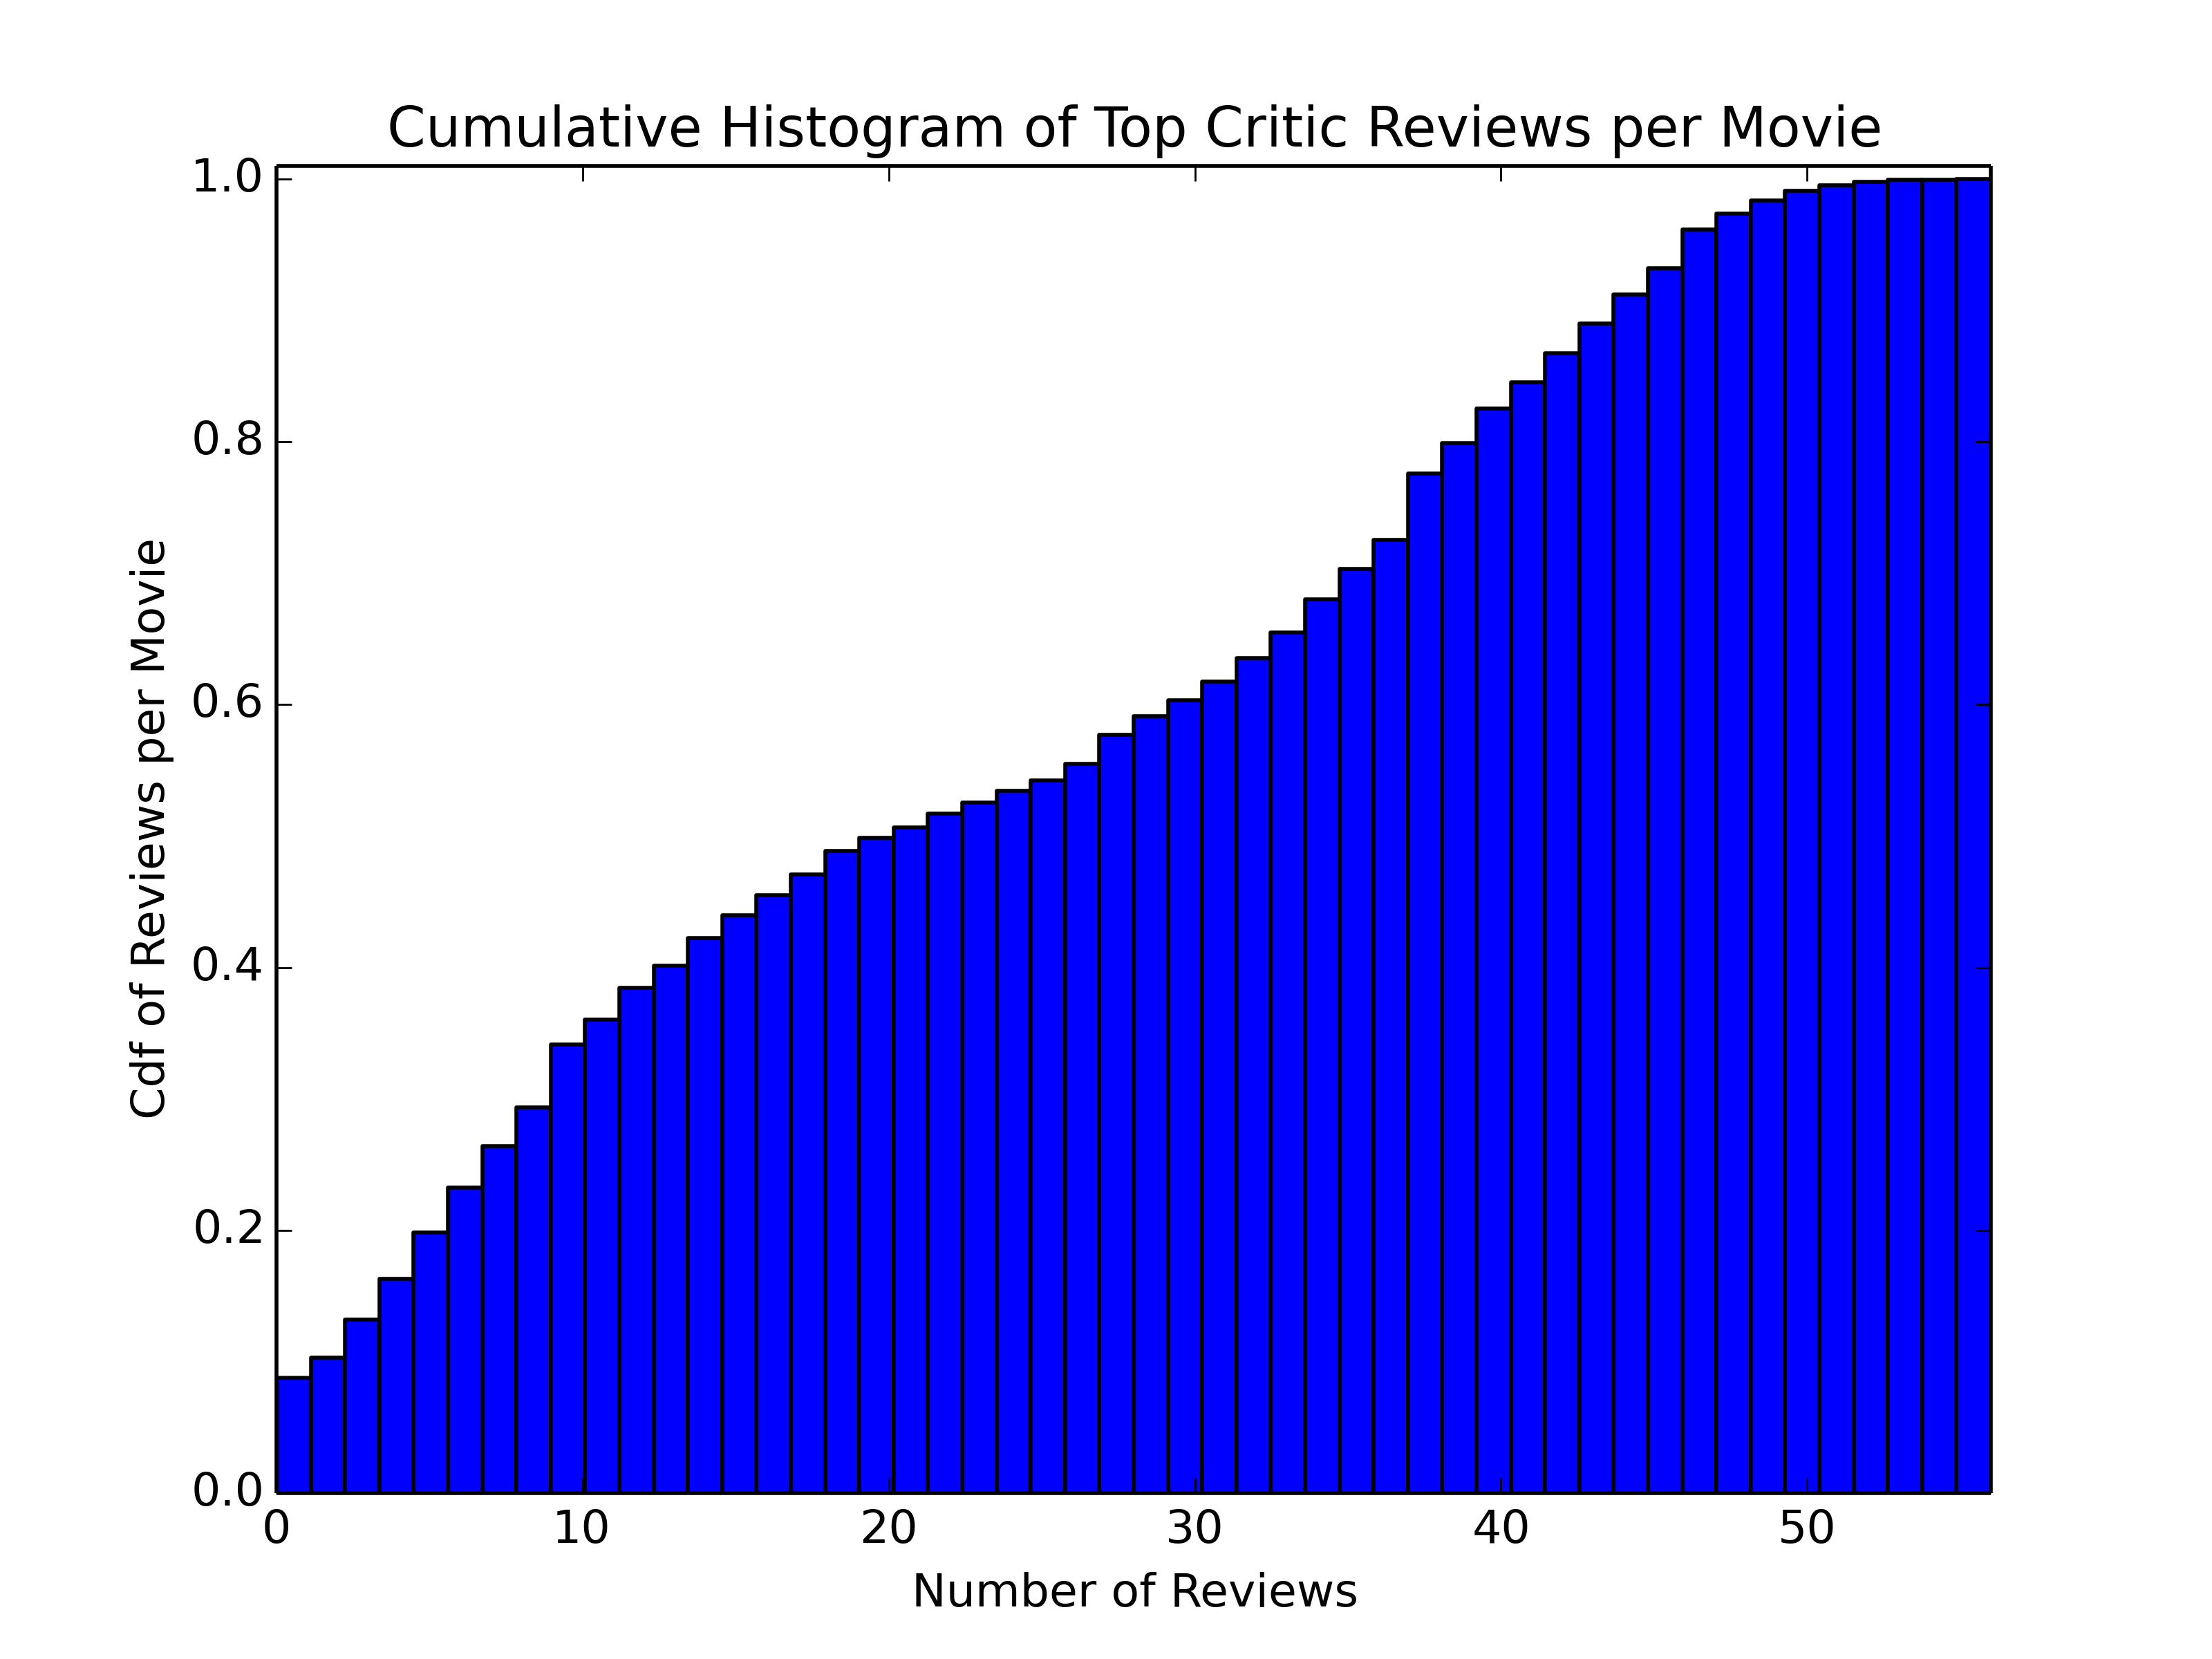
\includegraphics[width=0.44\textwidth, height=140px]{../plots/data/plot_r_mov_top.png}
    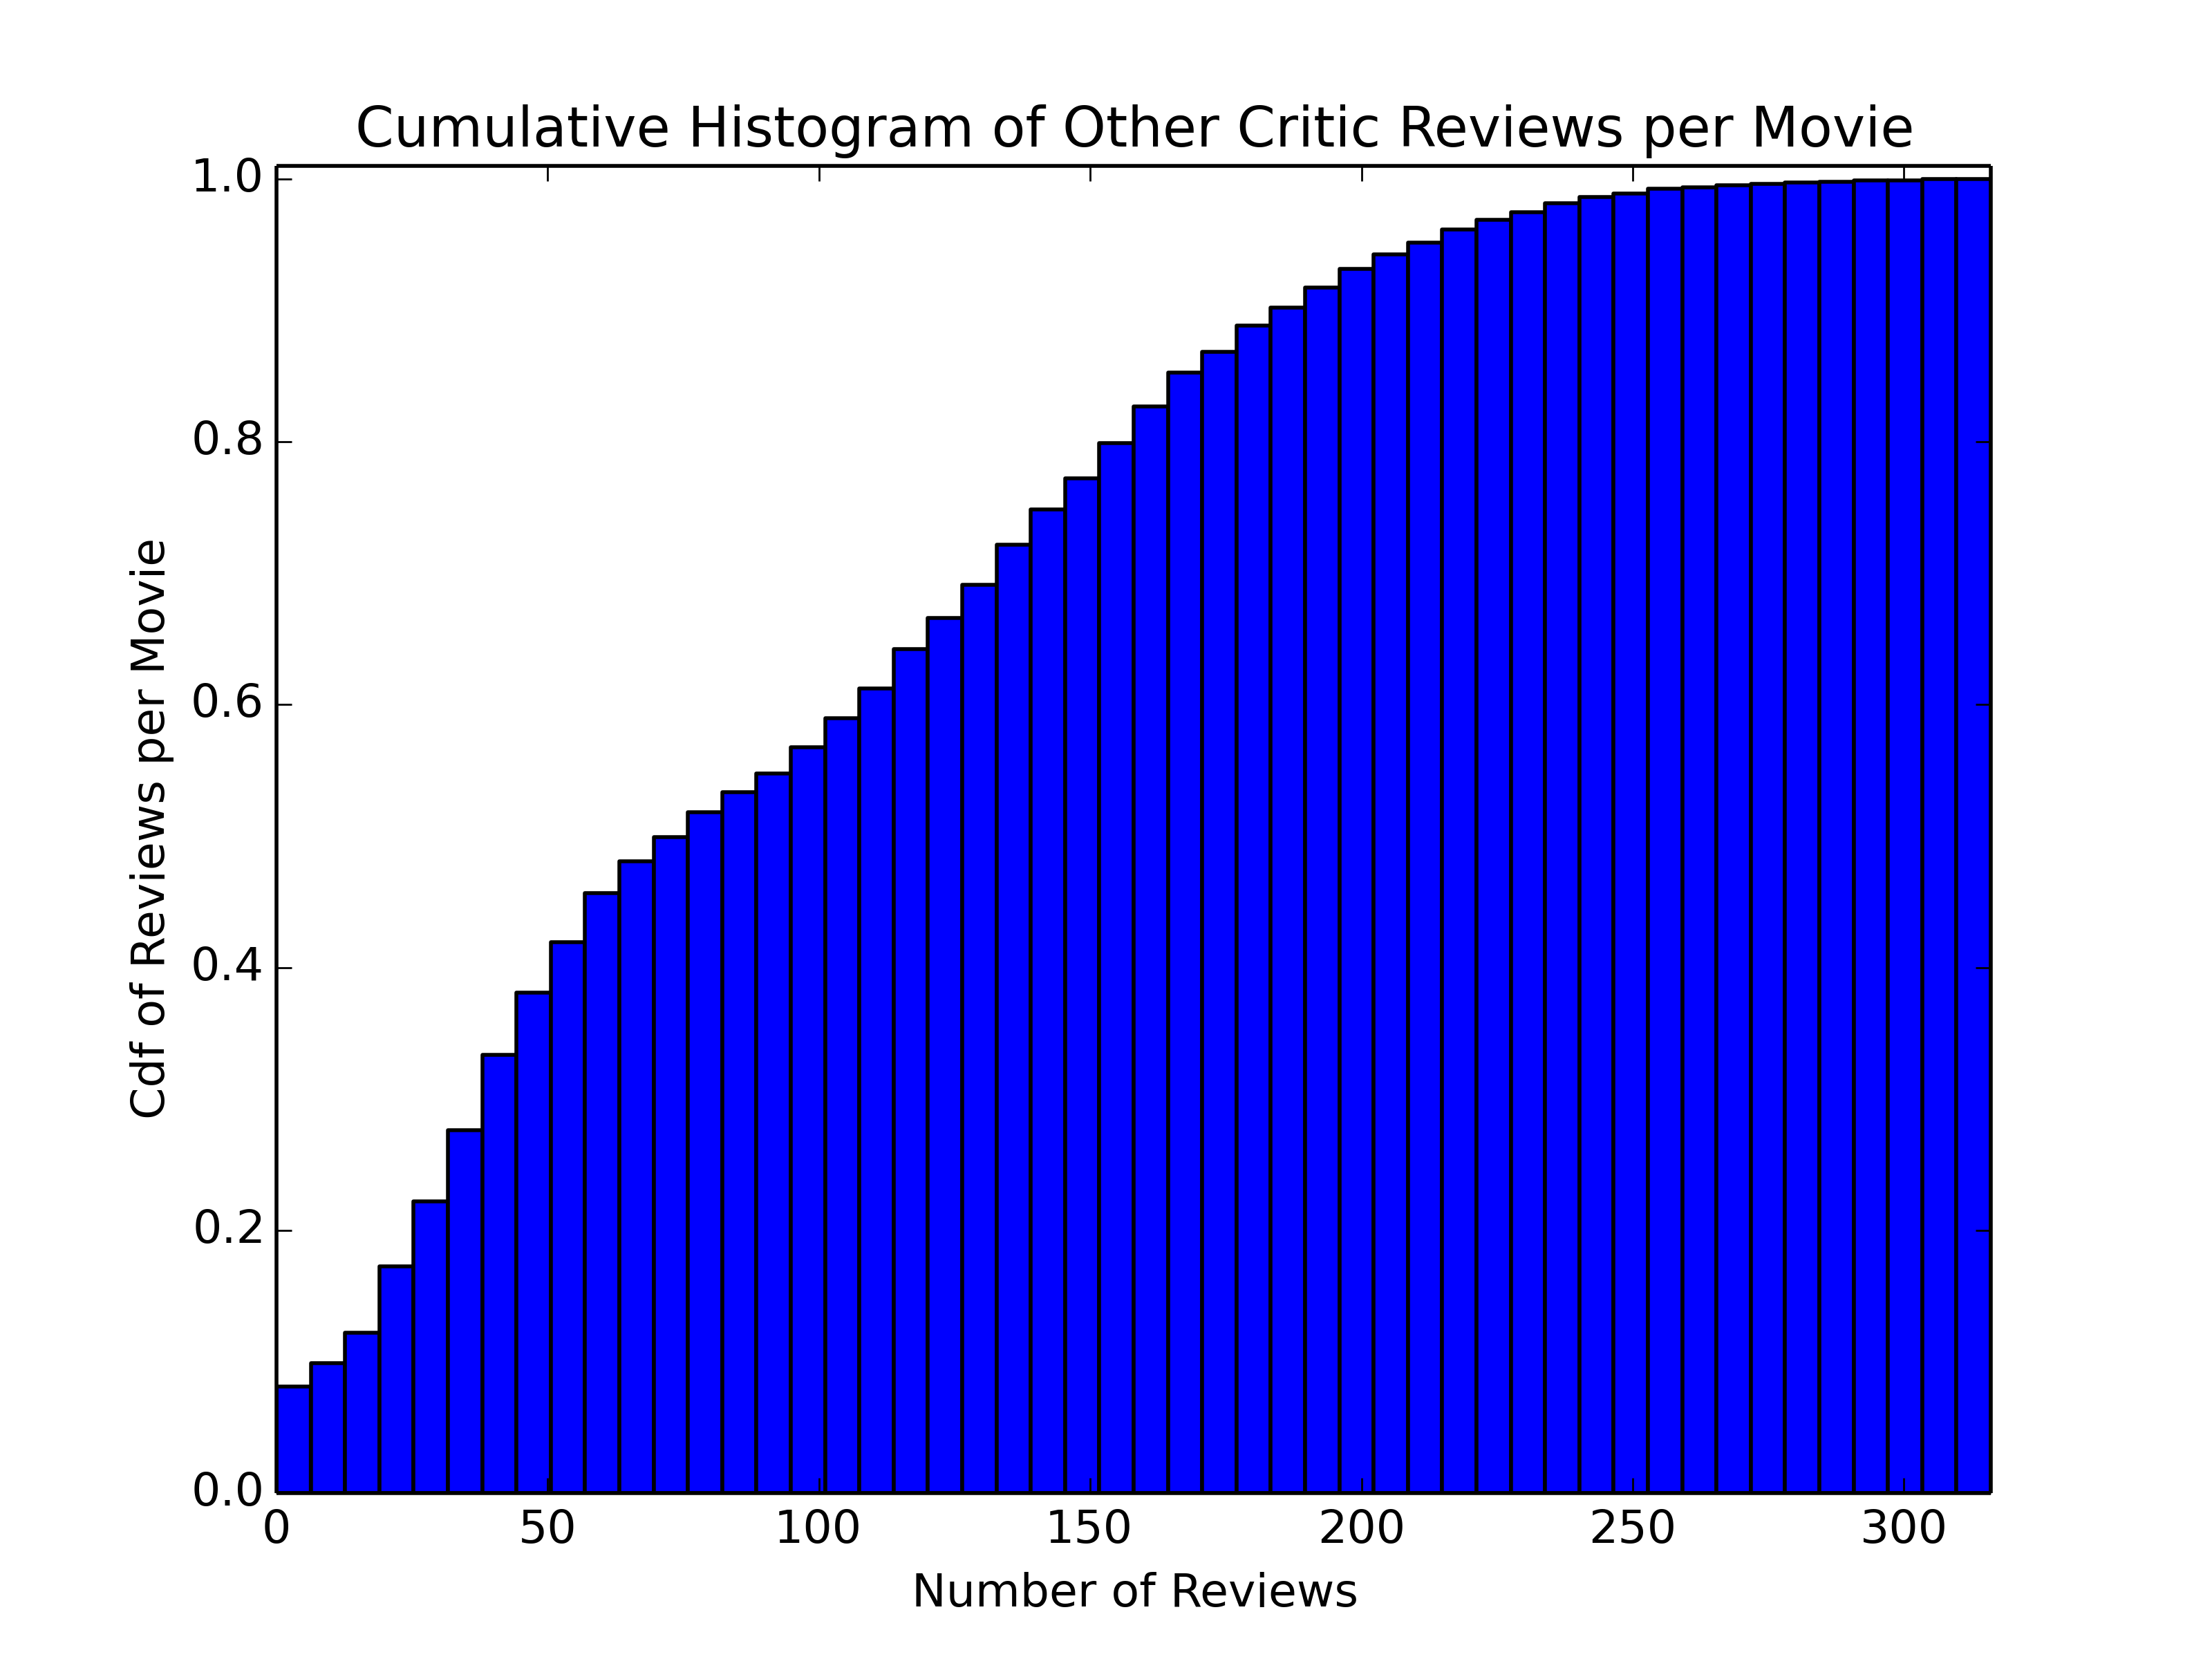
\includegraphics[width=0.44\textwidth, height=140px]{../plots/data/plot_r_mov_oth.png}
    \caption{Cumulative histograms of critic reviews per movie for movies on Rotten Tomatoes}
    \label{fig:r_mov} 
\end{figure}

\begin{figure}[H]
    \centering
    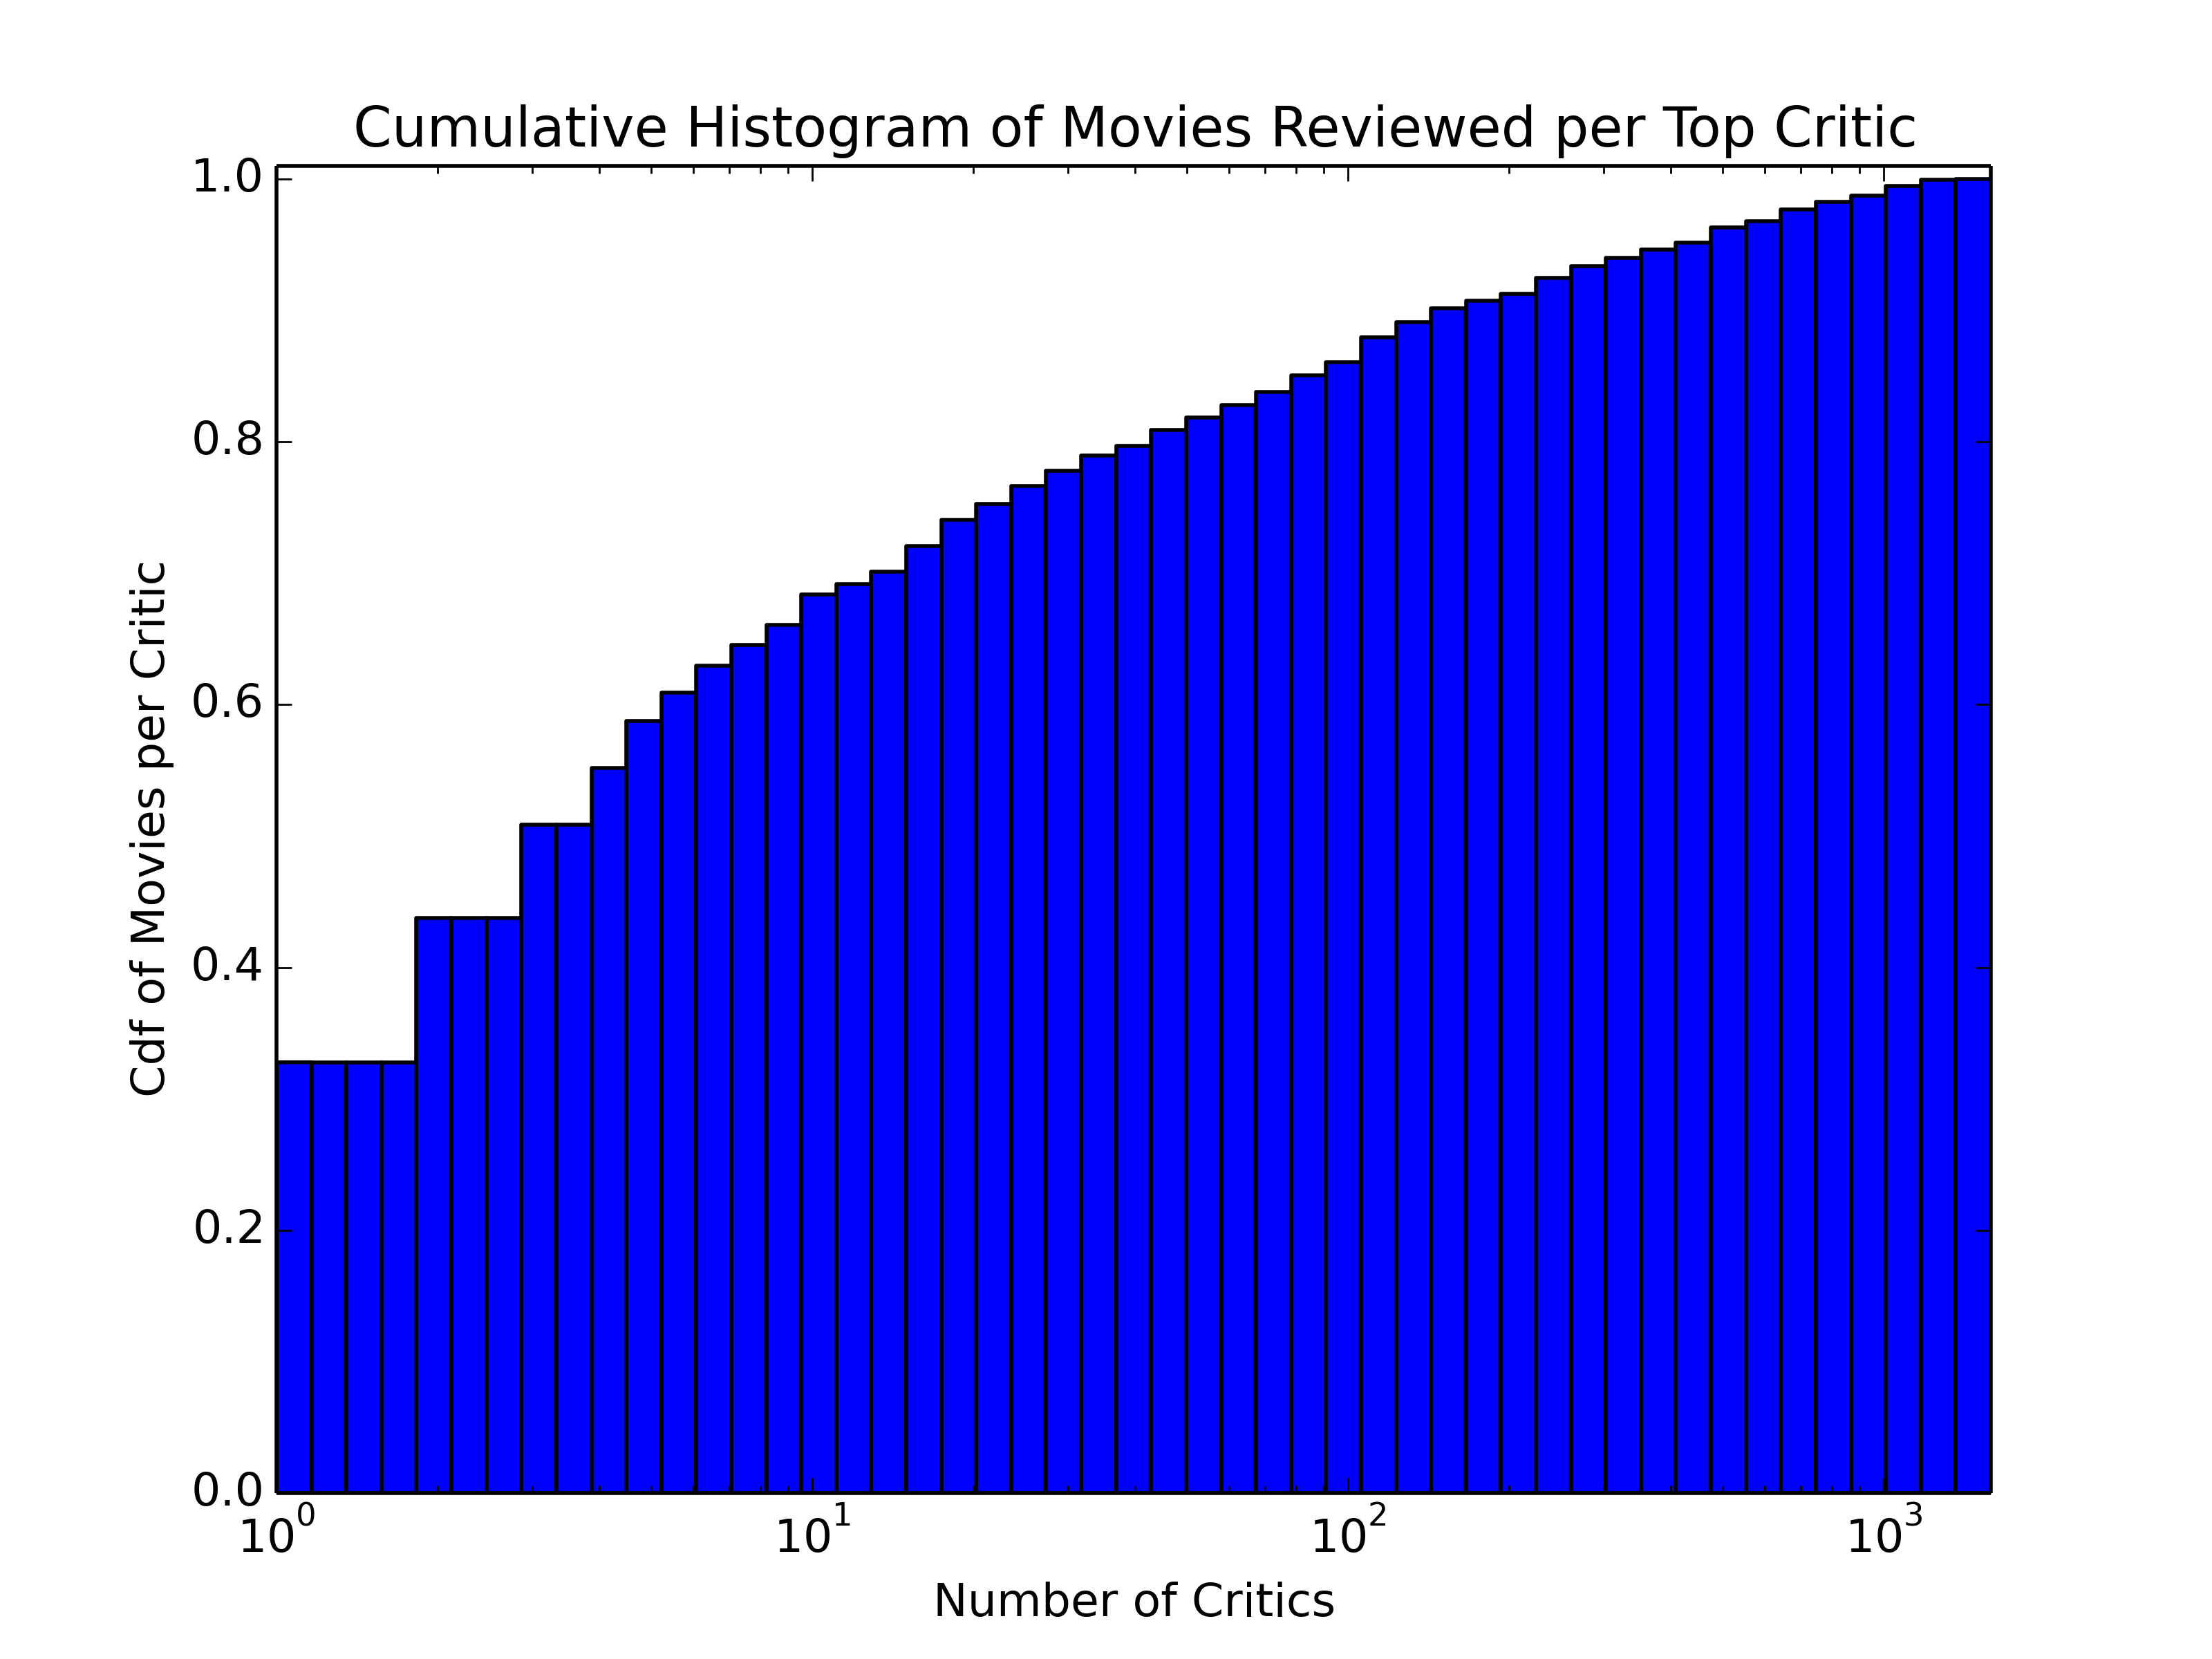
\includegraphics[width=0.44\textwidth, height=140px]{../plots/data/plot_r_crit_top.png}
    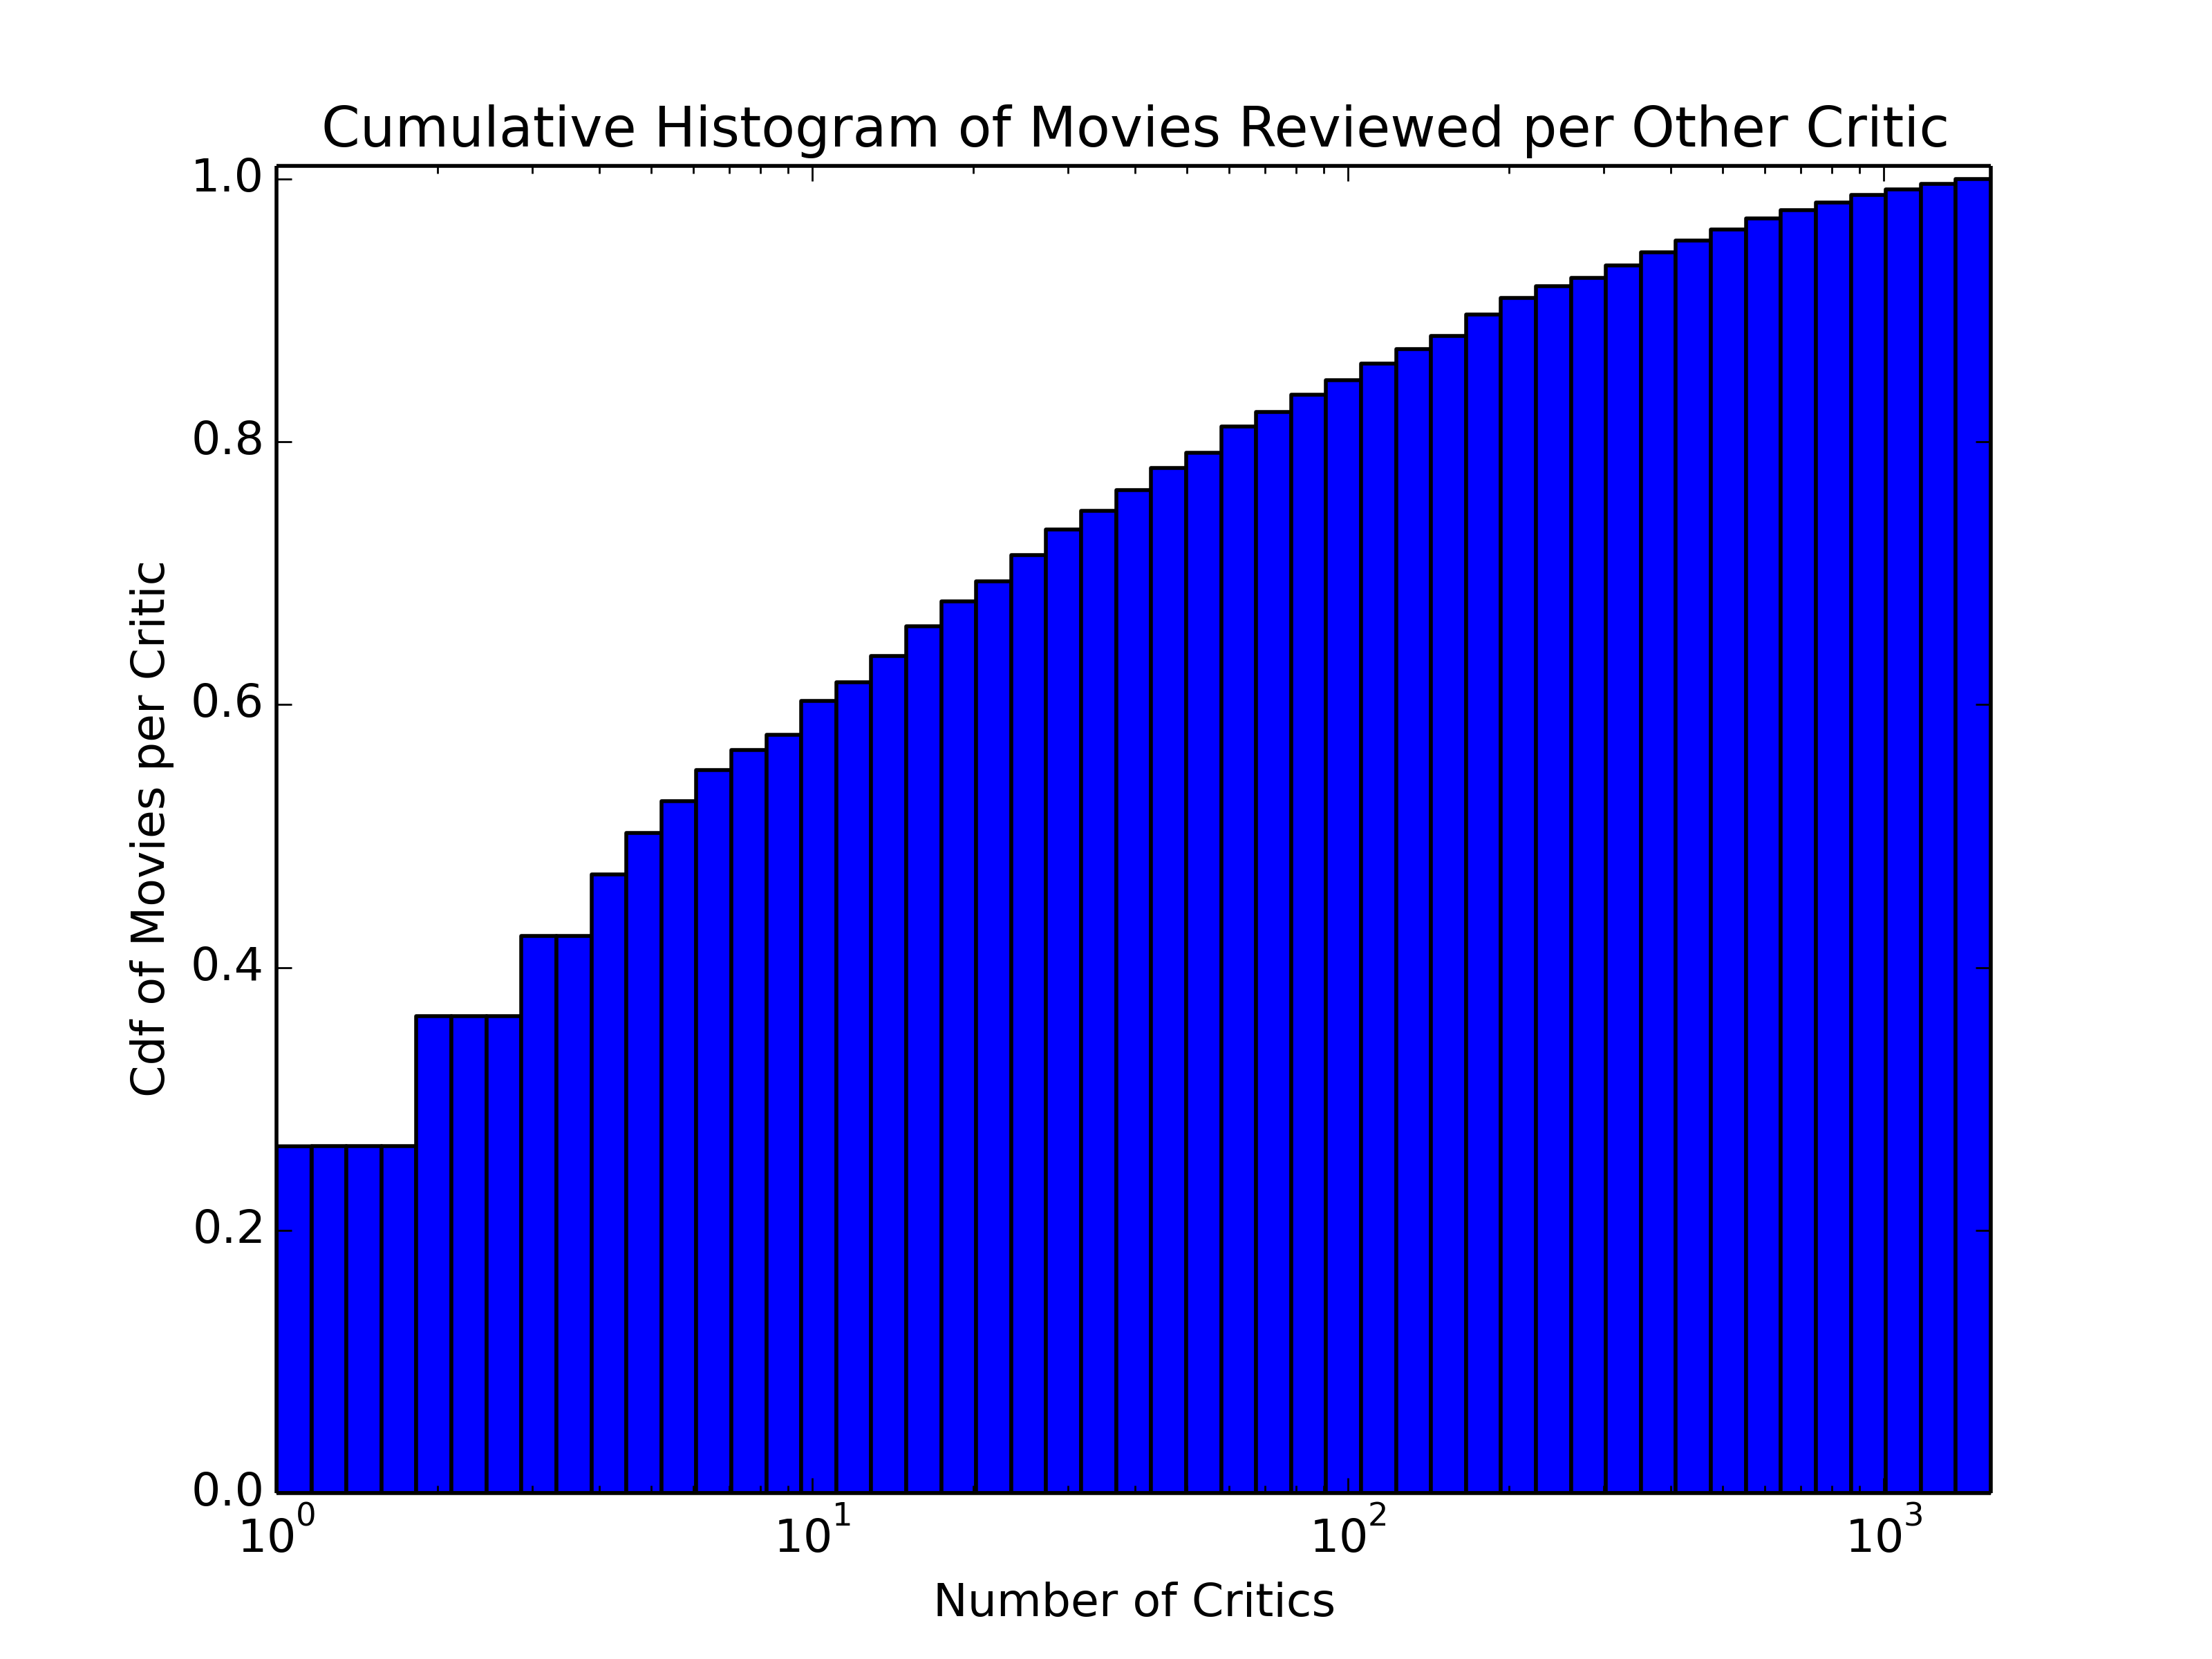
\includegraphics[width=0.44\textwidth, height=140px]{../plots/data/plot_r_crit_oth.png}
    \caption{Cumulative histograms of the number of movies reviewed by critics on Rotten Tomatoes}
    \label{fig:r_crit}
\end{figure}



\section{Matrix factorization results}

Figures \ref{fig:fac-d1} to \ref{fig:fac-d40} show some of the results we 
obtained with this technique. We first tried with only one dimension 
per user and critic $D=1$. As shown in Figure  \ref{fig:fac-d1}, this 
produces quite unimpressive results. This model is far too 
simple to learn anything particularly interesting. All we can really learn here 
is how lenient critics are, and the average rating given to a movie. This does 
give us some improvement over simply choosing the mean rating for each movie, 
which produces an average error of $20$. Also, even with no regularization we 
overfit very little.

As we increase the number of features, we see that our training and test error 
both improve. However, as this occurs the training and test error become less 
correlated. With a larger number of dimensions we become more vulnerable to 
over fitting, and the regularization parameter $\lambda$ becomes 
increasingly important. This is particularly notable in Figures 
\ref{fig:fac-d40} and \ref{fig:fac-d25} where the test error quickly diverges
unless the largest regularization constant $\lambda = 1000$ is used.

It is interesting that when the matrix factorization eventually overfits 
badly, as in the first diagram of Figure \ref{fig:fac-d40}, the graph of 
Error vs. Iteration looks like a standard bias-variance tradeoff. Although 
at first this seems unintuitive at first, it makes sense when we consider that 
iterations is a measure of model complexity. With few iterations, even with 
many dimensions, it is not possible to reach all that many configurations. 
It would be interesting to see how an iteration dependent regularization 
constant performs. 

The best test error seems to occur in the most complex model with the highest 
regularization constant $D=40$, $\lambda = 1000$. Here our model achieves an 
error of approximately \matrixtesterror.

\begin{figure}[H]
\centering
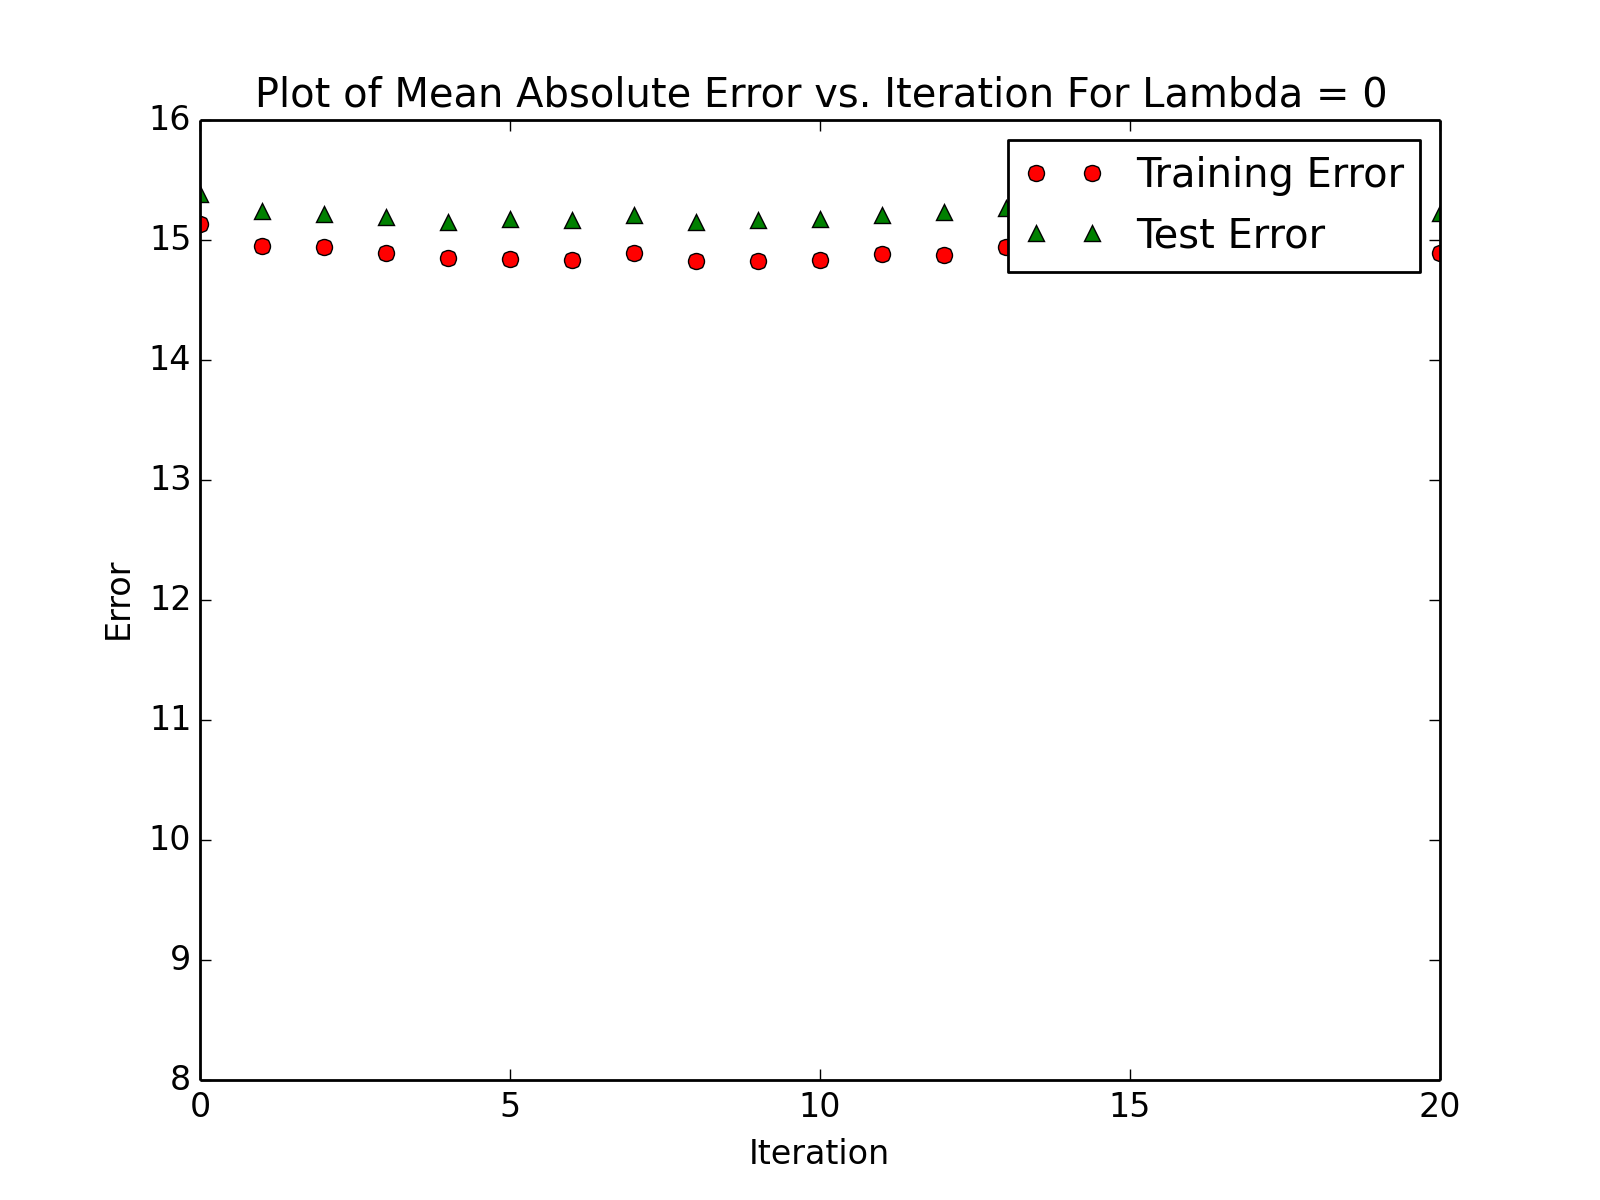
\includegraphics[width=0\factwidth\textwidth,height=\factheight]{matrix_plots/test-i40d1l0.png}
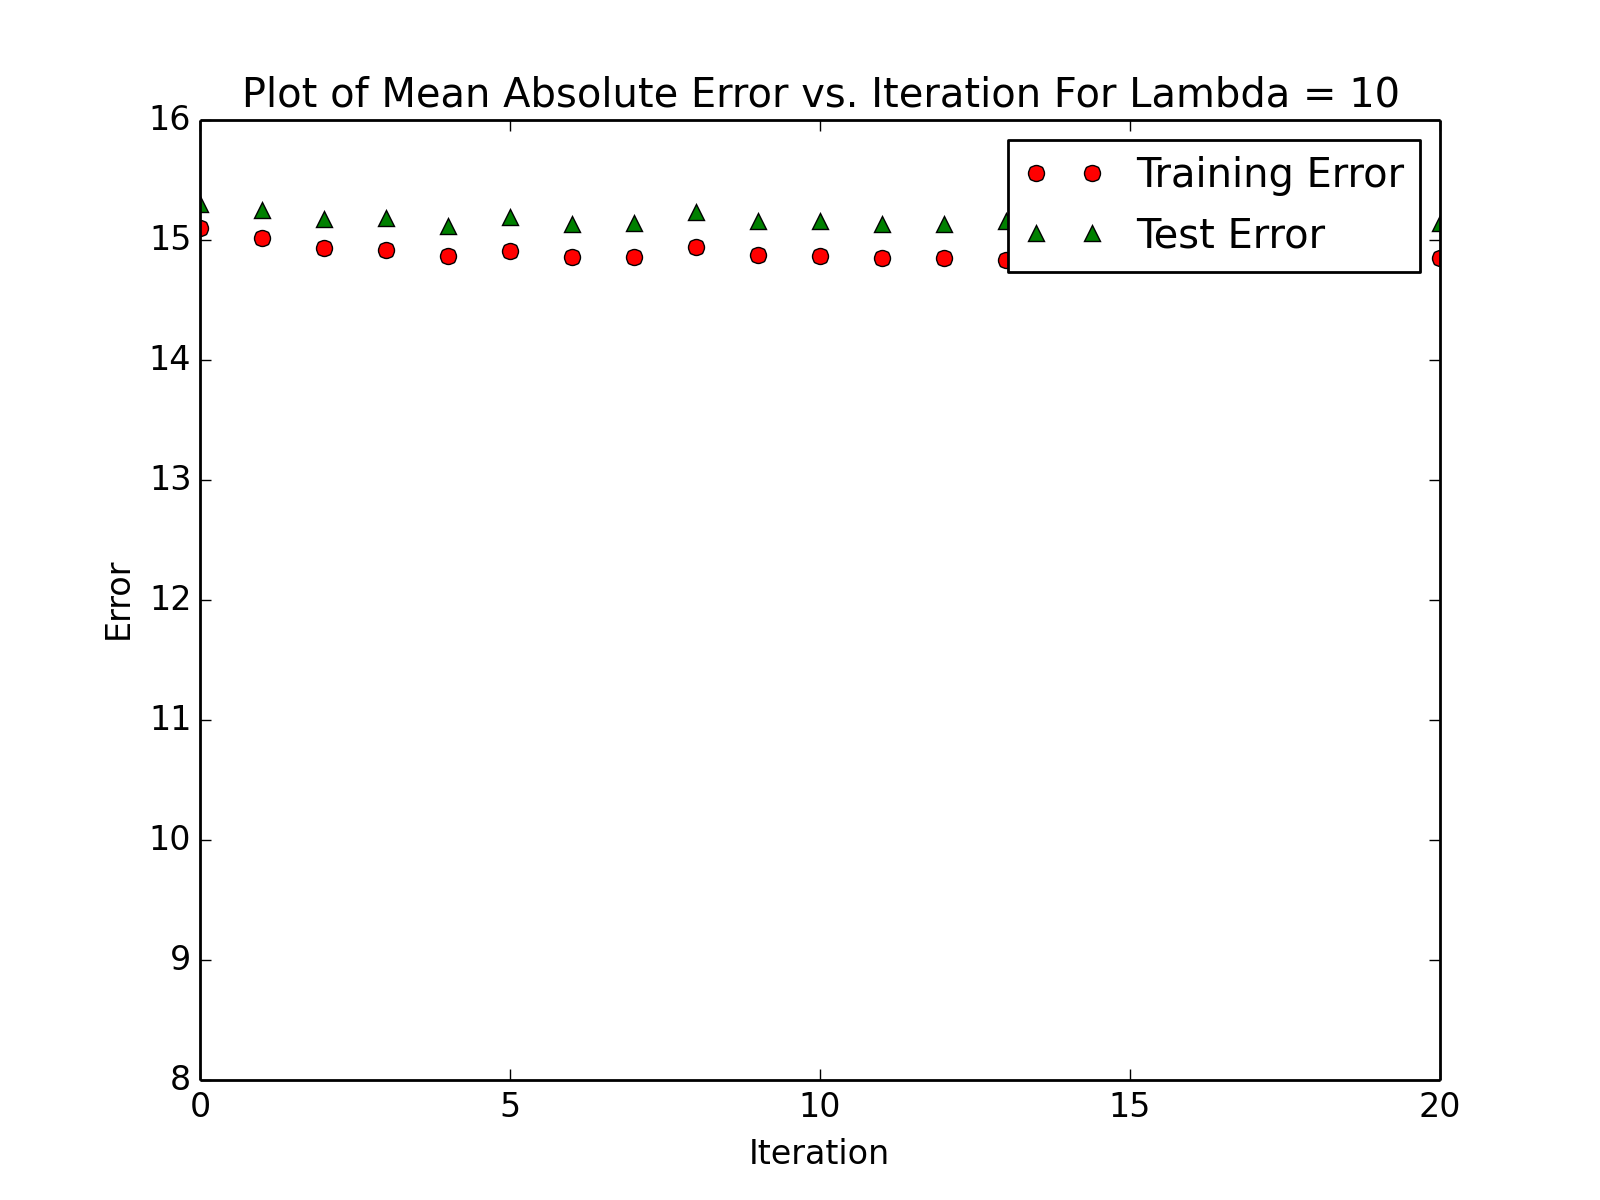
\includegraphics[width=0\factwidth\textwidth,height=\factheight]{matrix_plots/test-i40d1l10.png}
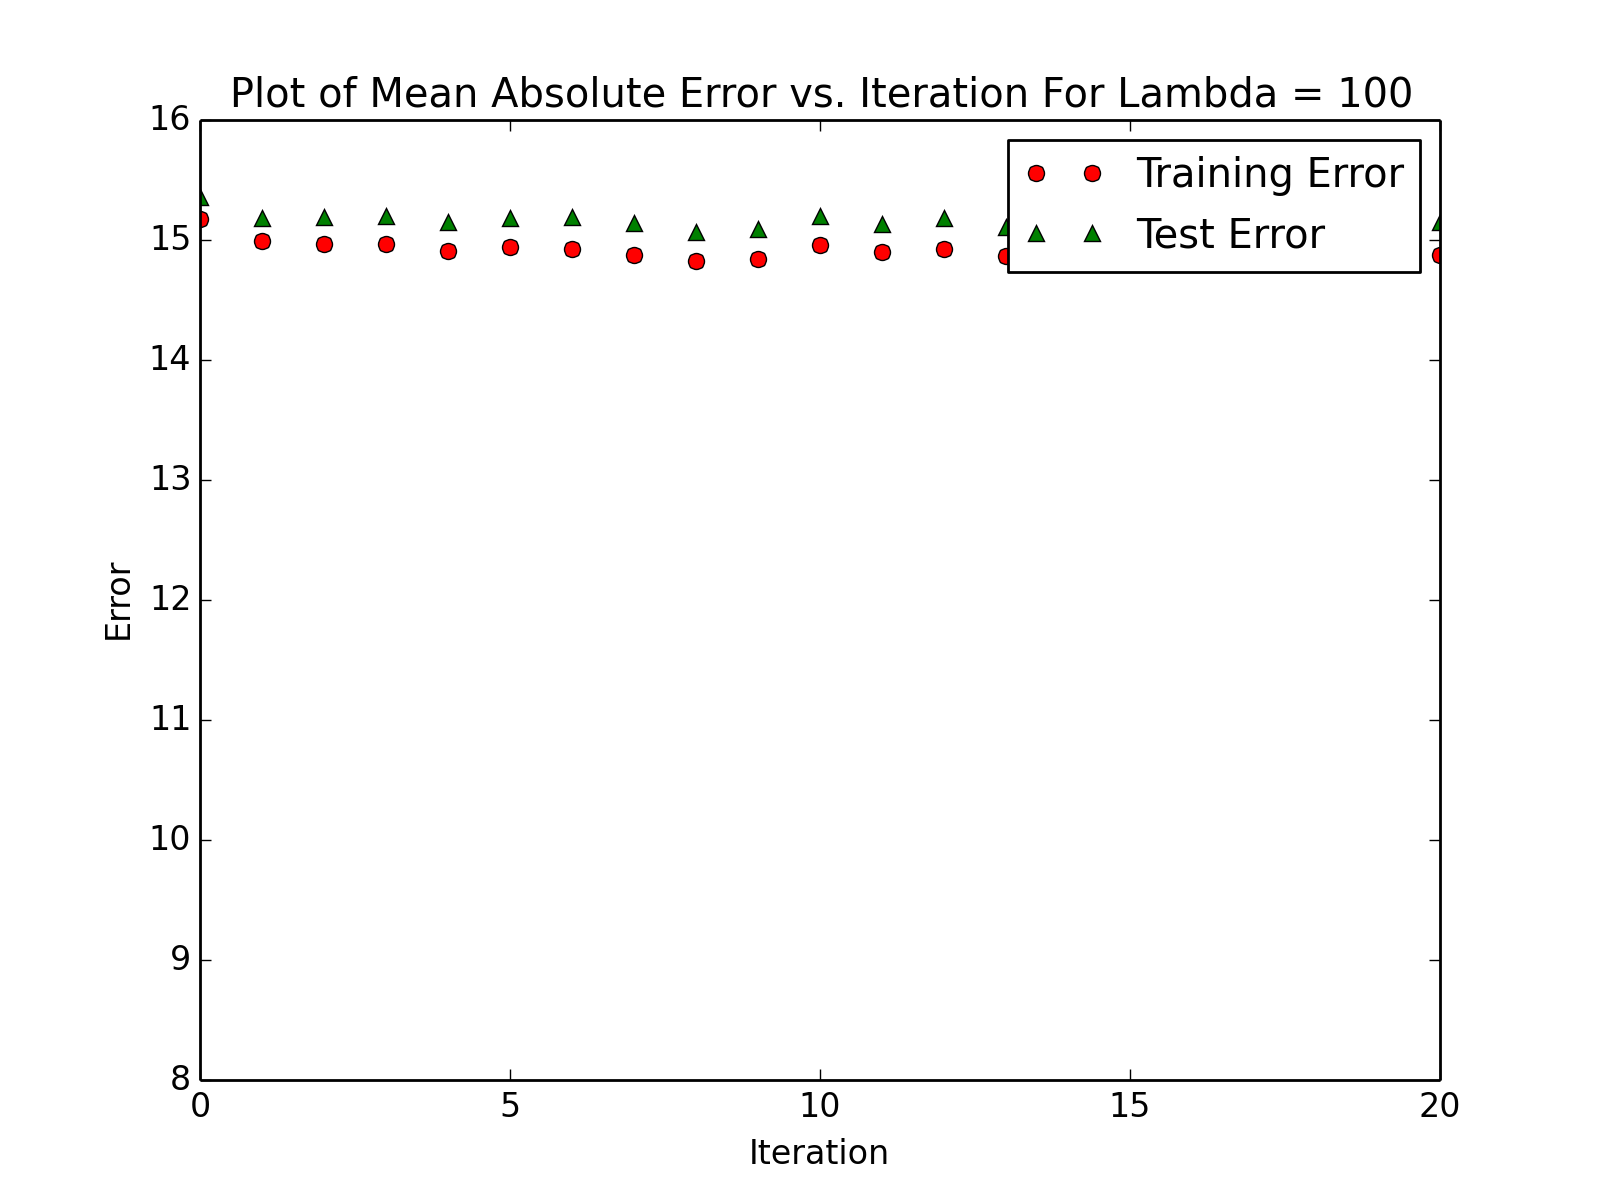
\includegraphics[width=0\factwidth\textwidth,height=\factheight]{matrix_plots/test-i40d1l100.png}
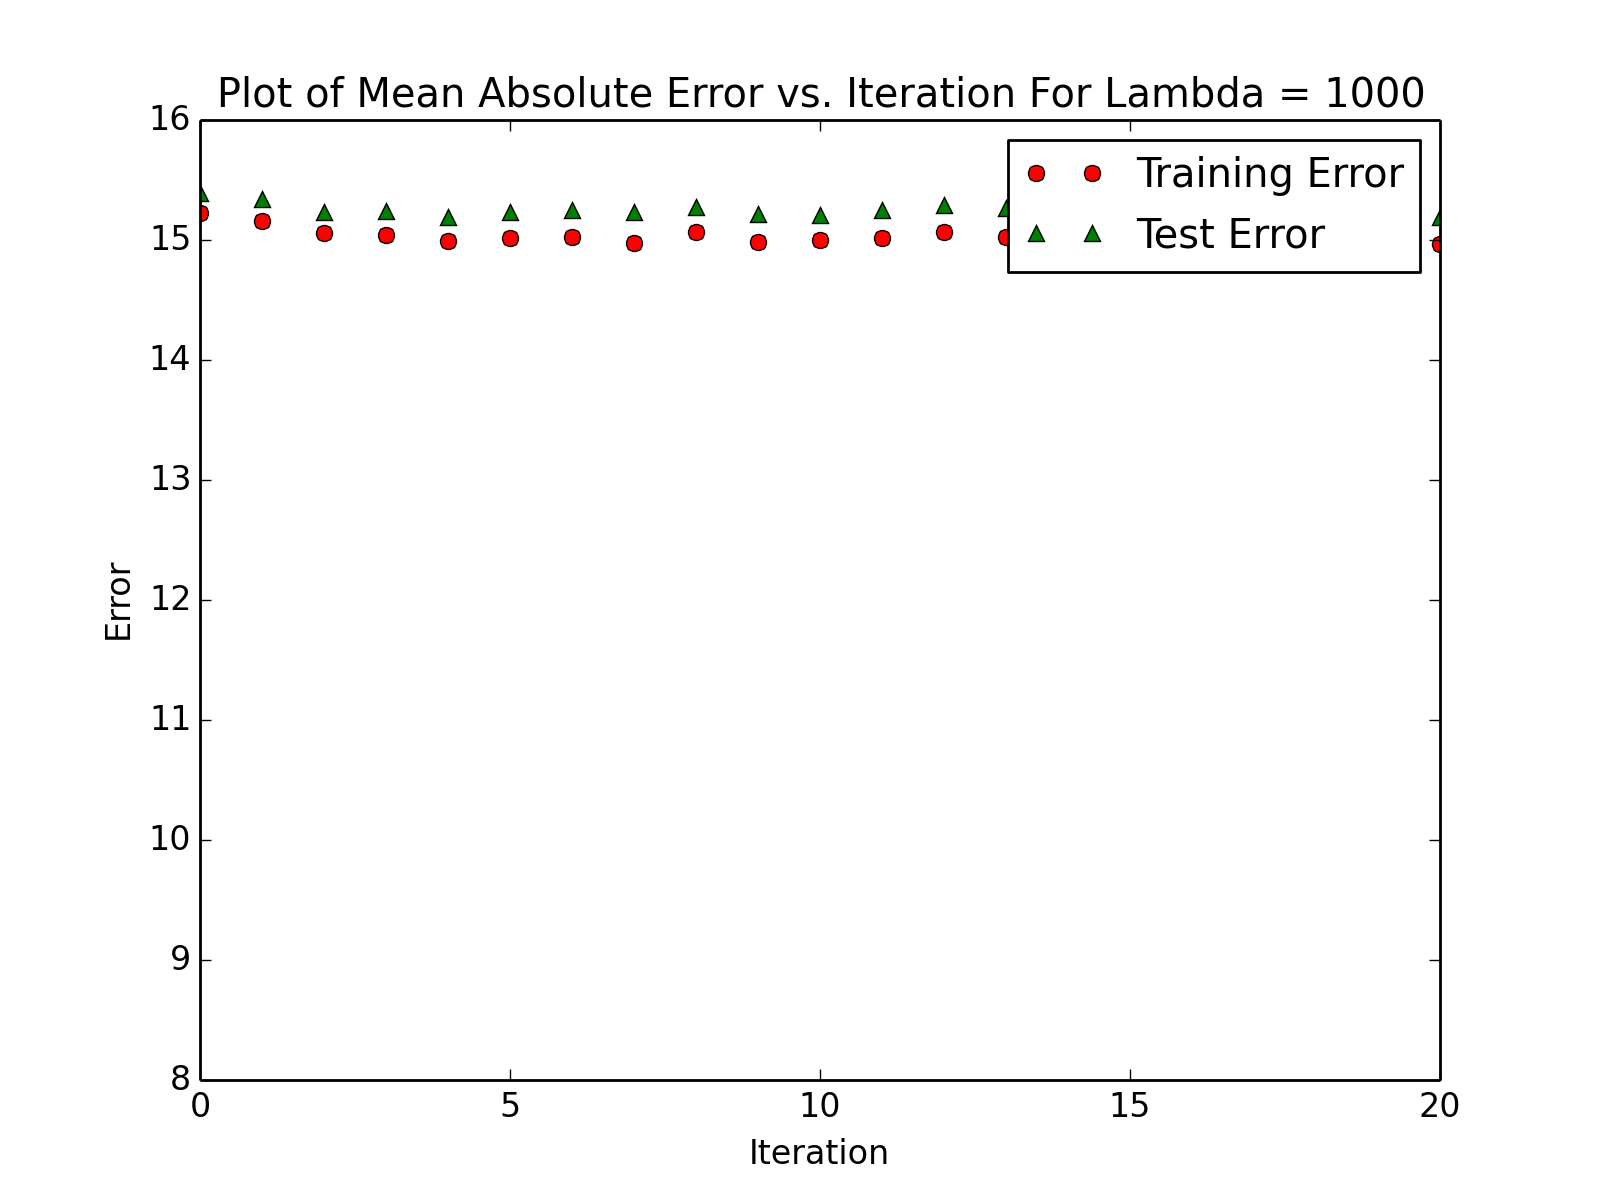
\includegraphics[width=0\factwidth\textwidth,height=\factheight]{matrix_plots/test-i40d1l1000.png}
\caption{Mean absolute training and test error over 20 iterations in the stochastic matrix factorization model. Stocastic gradient descent was performed using a step size of 0.002. The learned critic matrix was count(critics) by 1, and the learned movie matrix was 1 by count(movies).}
\label{fig:fac-d1}
\end{figure}
\begin{figure}[H]
\centering
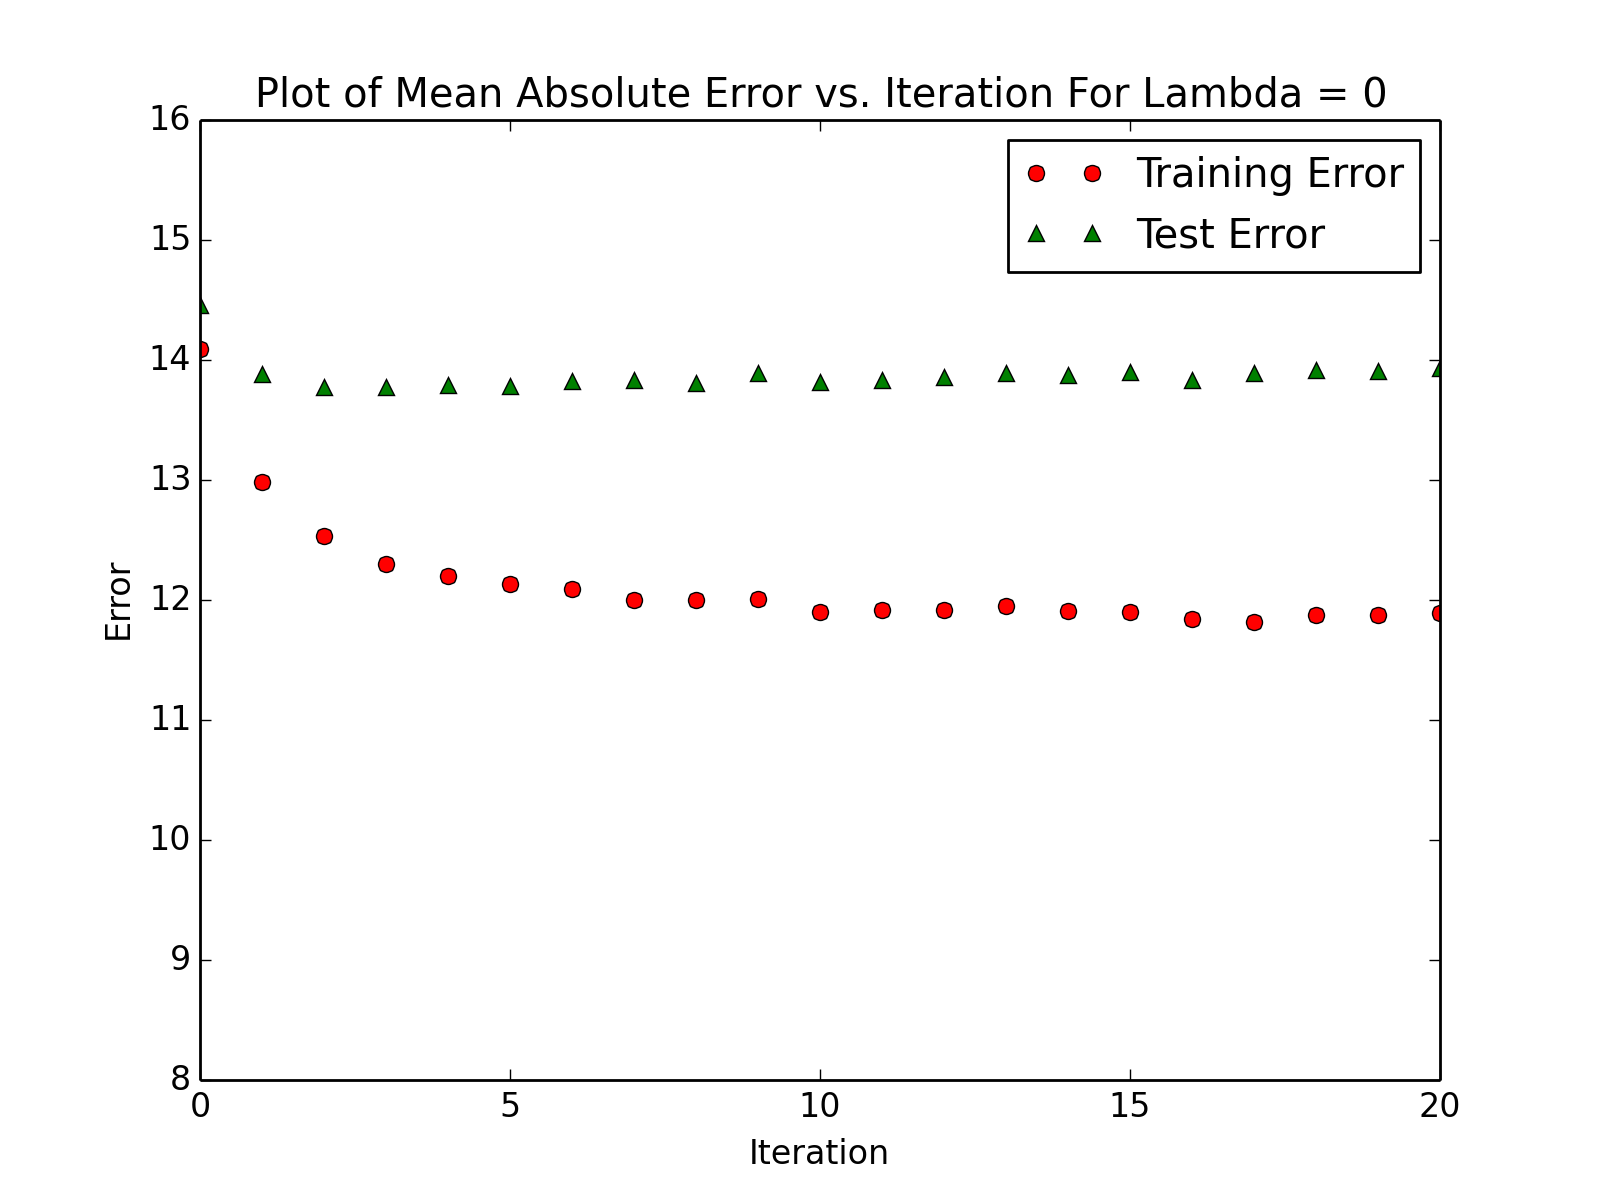
\includegraphics[width=0\factwidth\textwidth,height=\factheight]{matrix_plots/test-i40d10l0.png}
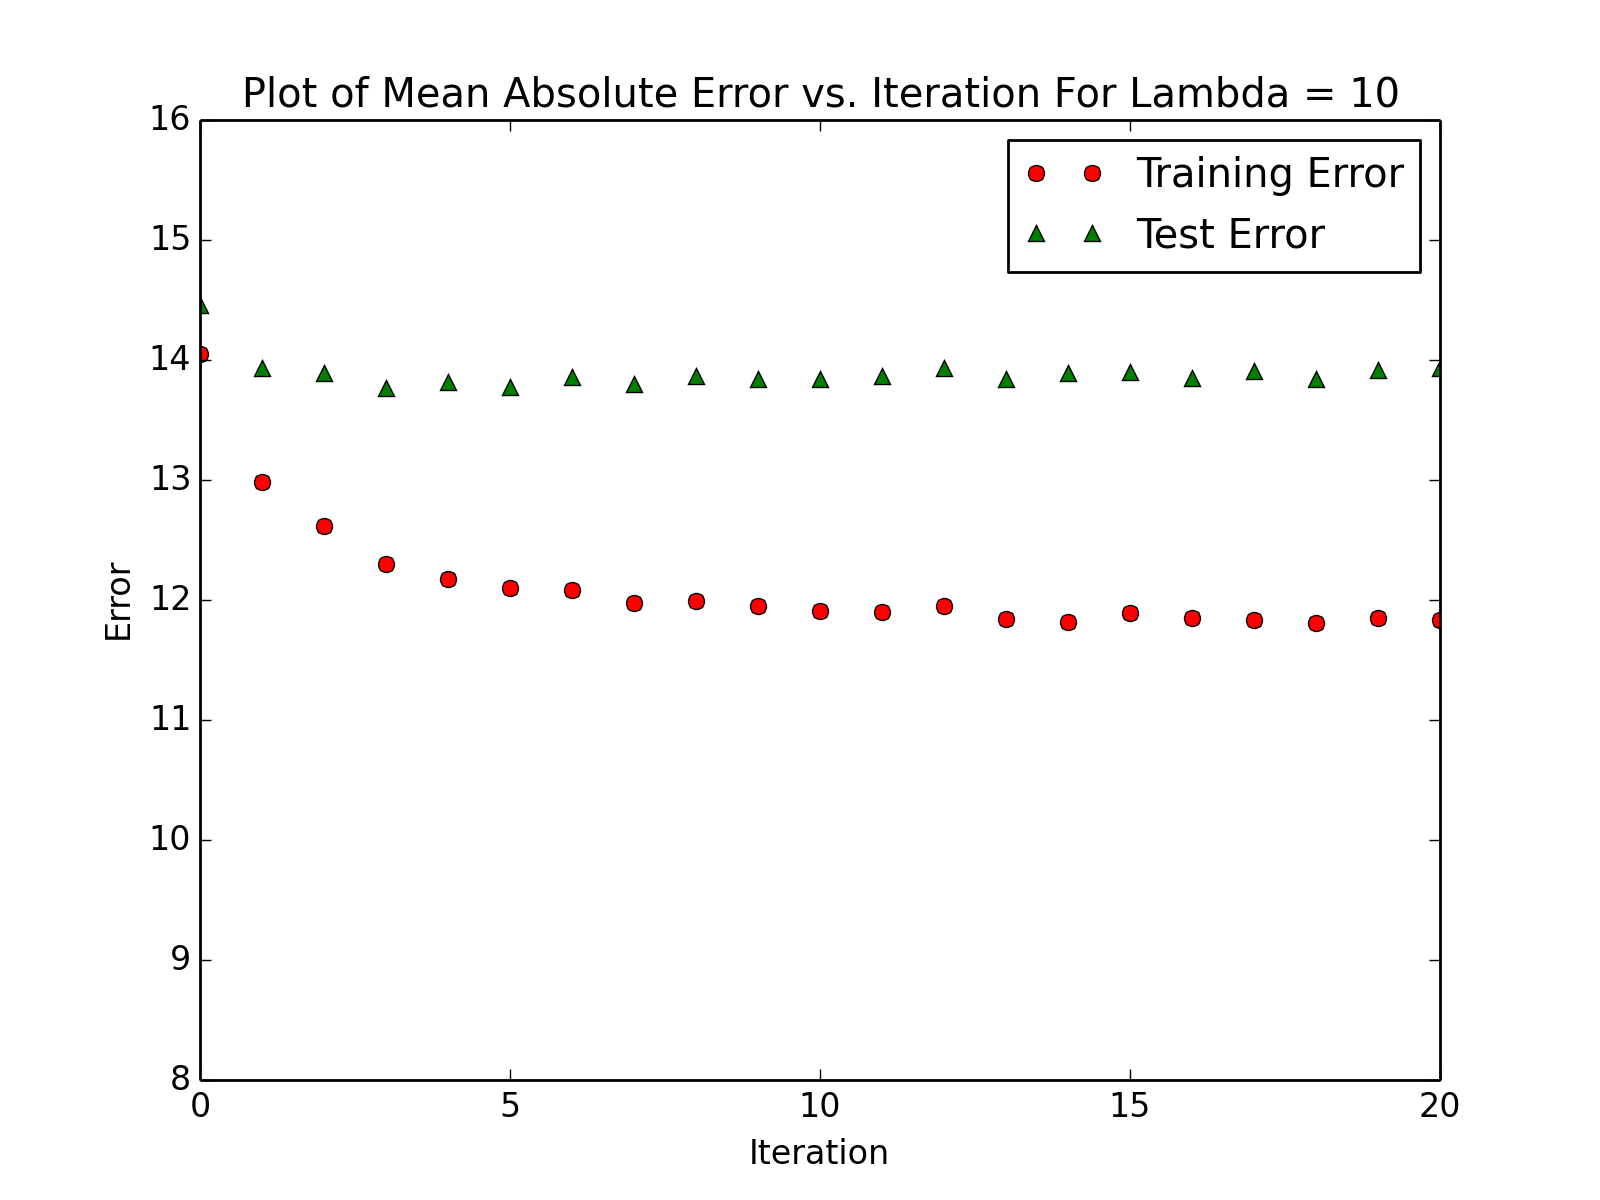
\includegraphics[width=0\factwidth\textwidth,height=\factheight]{matrix_plots/test-i40d10l10.png}
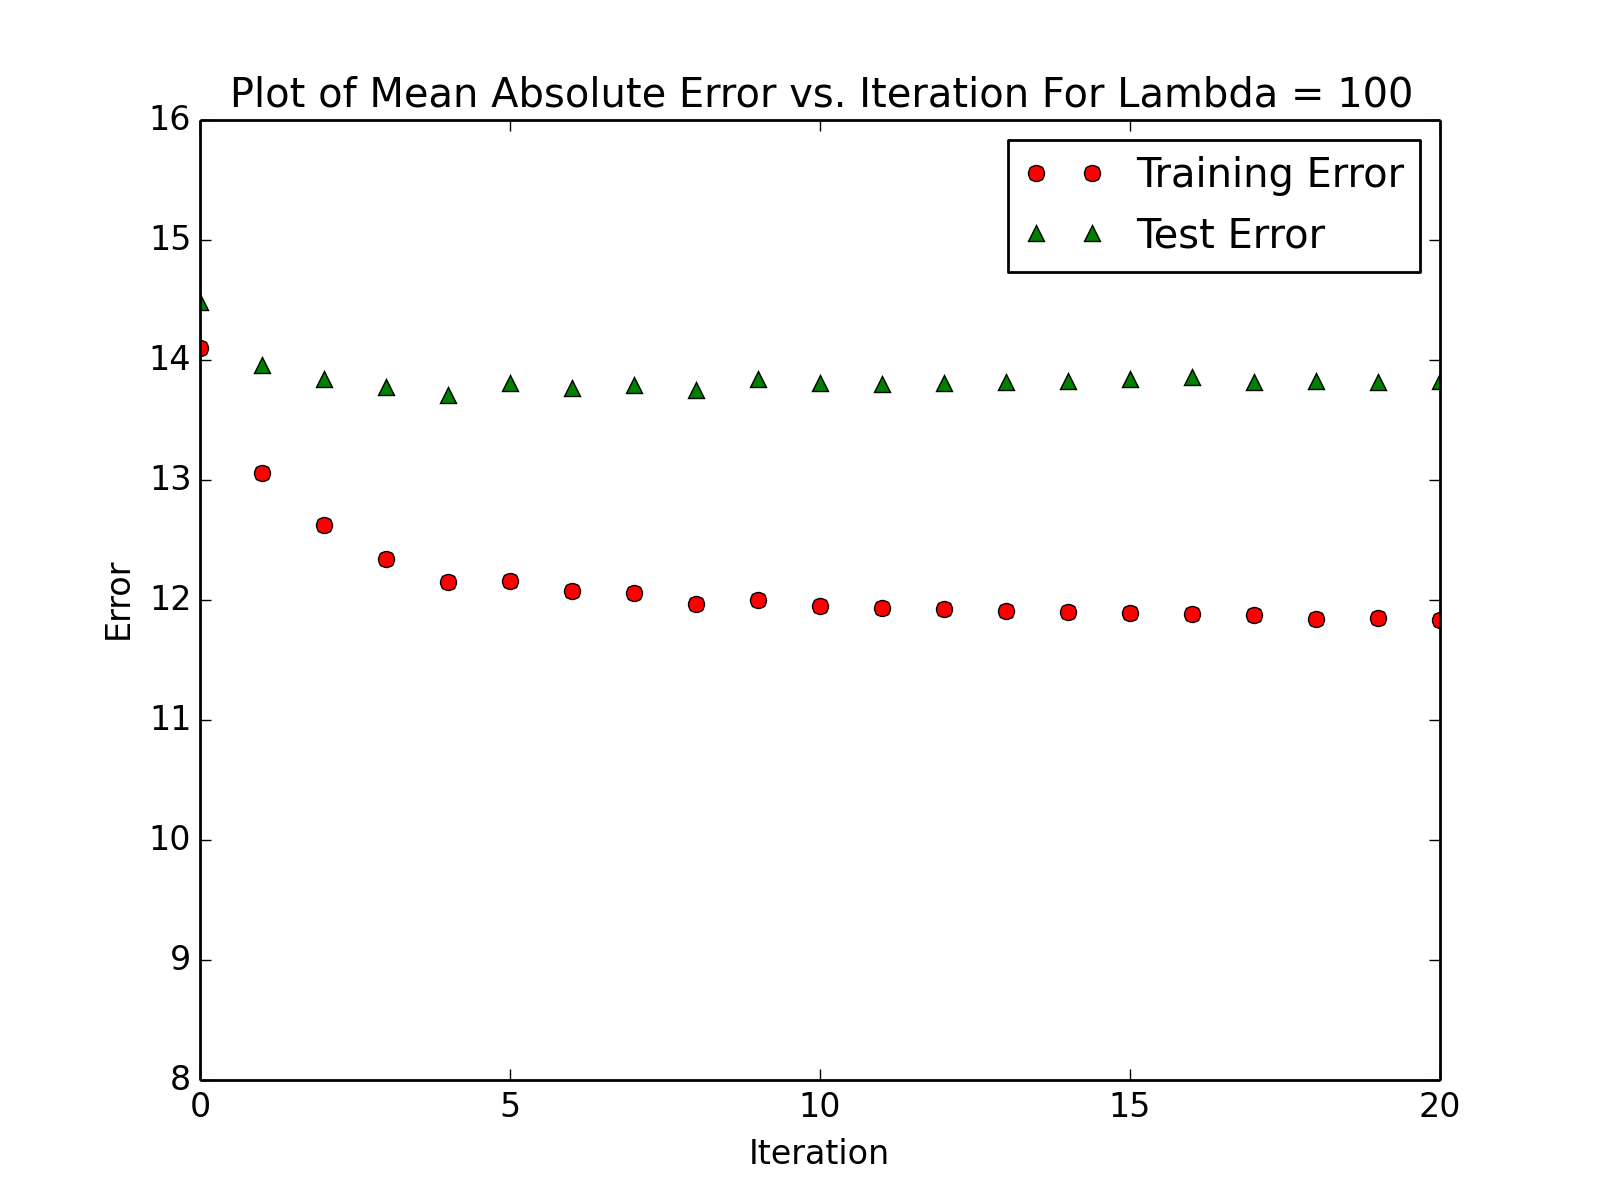
\includegraphics[width=0\factwidth\textwidth,height=\factheight]{matrix_plots/test-i40d10l100.png}
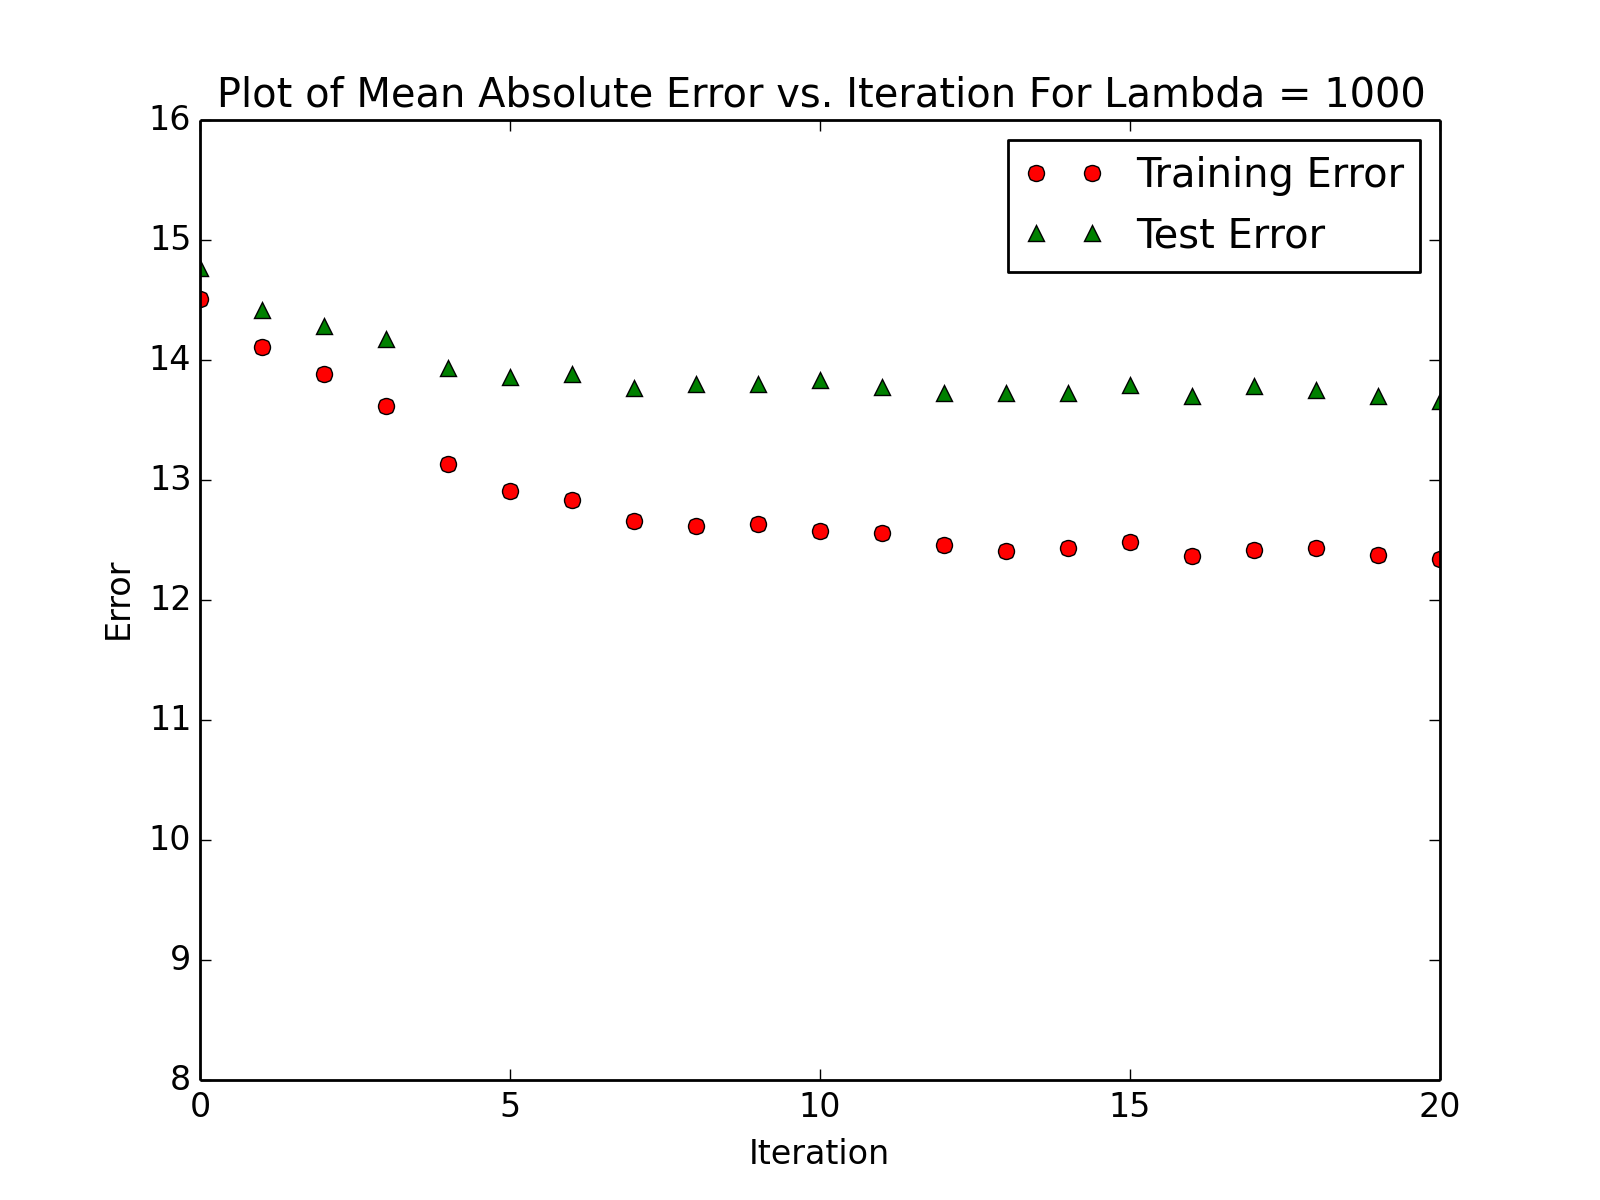
\includegraphics[width=0\factwidth\textwidth,height=\factheight]{matrix_plots/test-i40d10l1000.png}
\caption{Mean absolute training and test error over 20 iterations in the stochastic matrix factorization model. Stocastic gradient descent was performed using a step size of 0.002. The learned critic matrix was count(critics) by 10, and the learned movie matrix was 10 by count(movies).}
\label{fig:fac-d10}
\end{figure}
\begin{figure}[H]
\centering
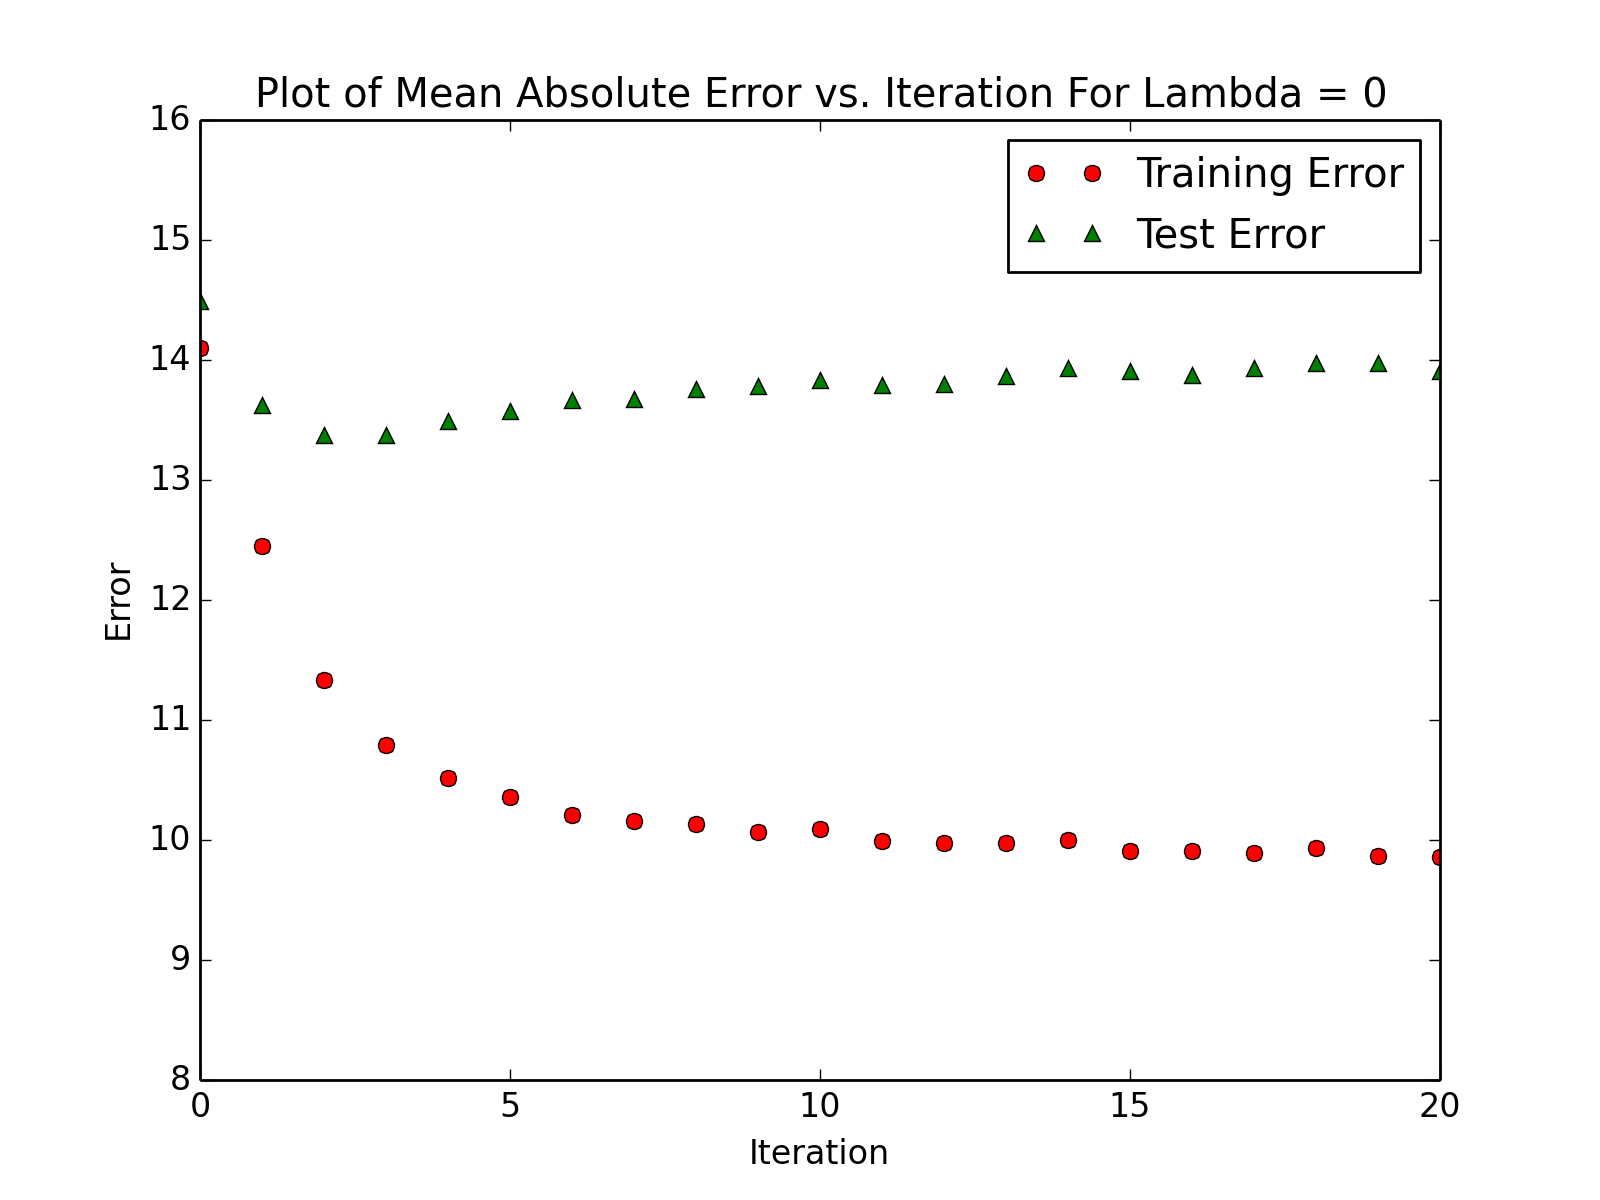
\includegraphics[width=0\factwidth\textwidth,height=\factheight]{matrix_plots/test-i40d25l0.png}
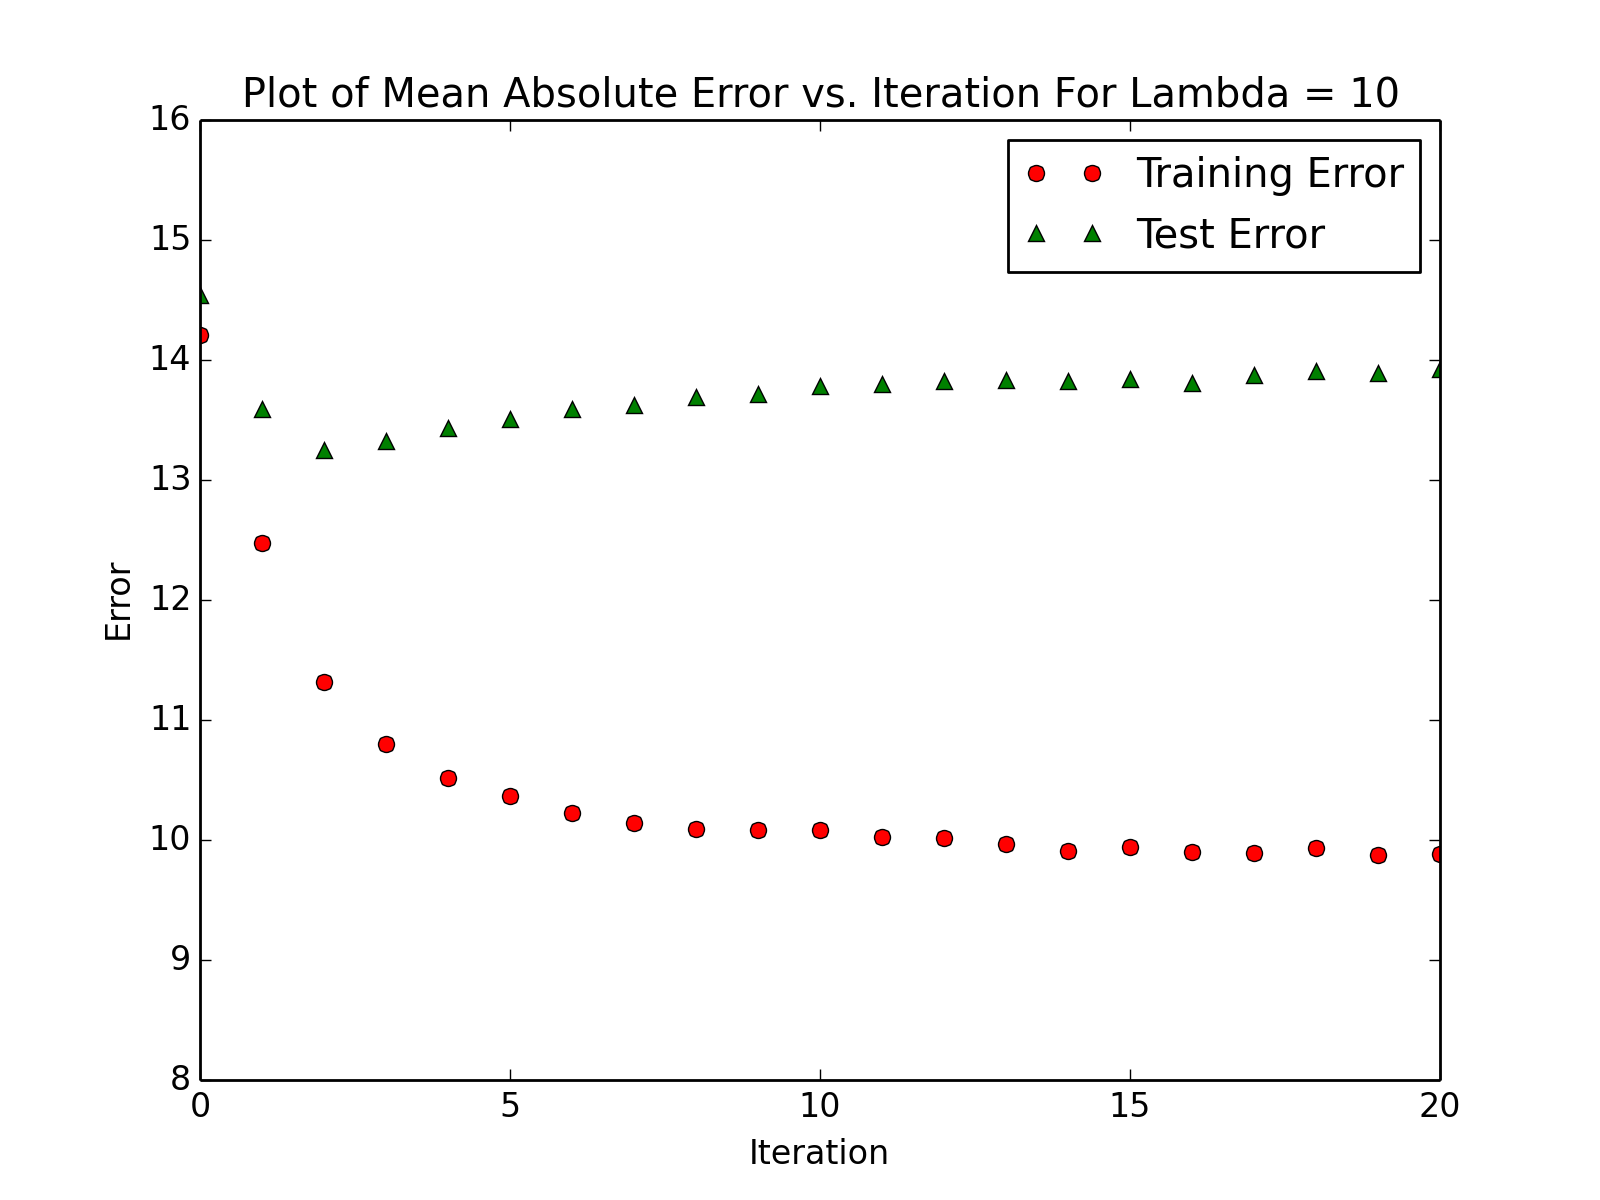
\includegraphics[width=0\factwidth\textwidth,height=\factheight]{matrix_plots/test-i40d25l10.png}
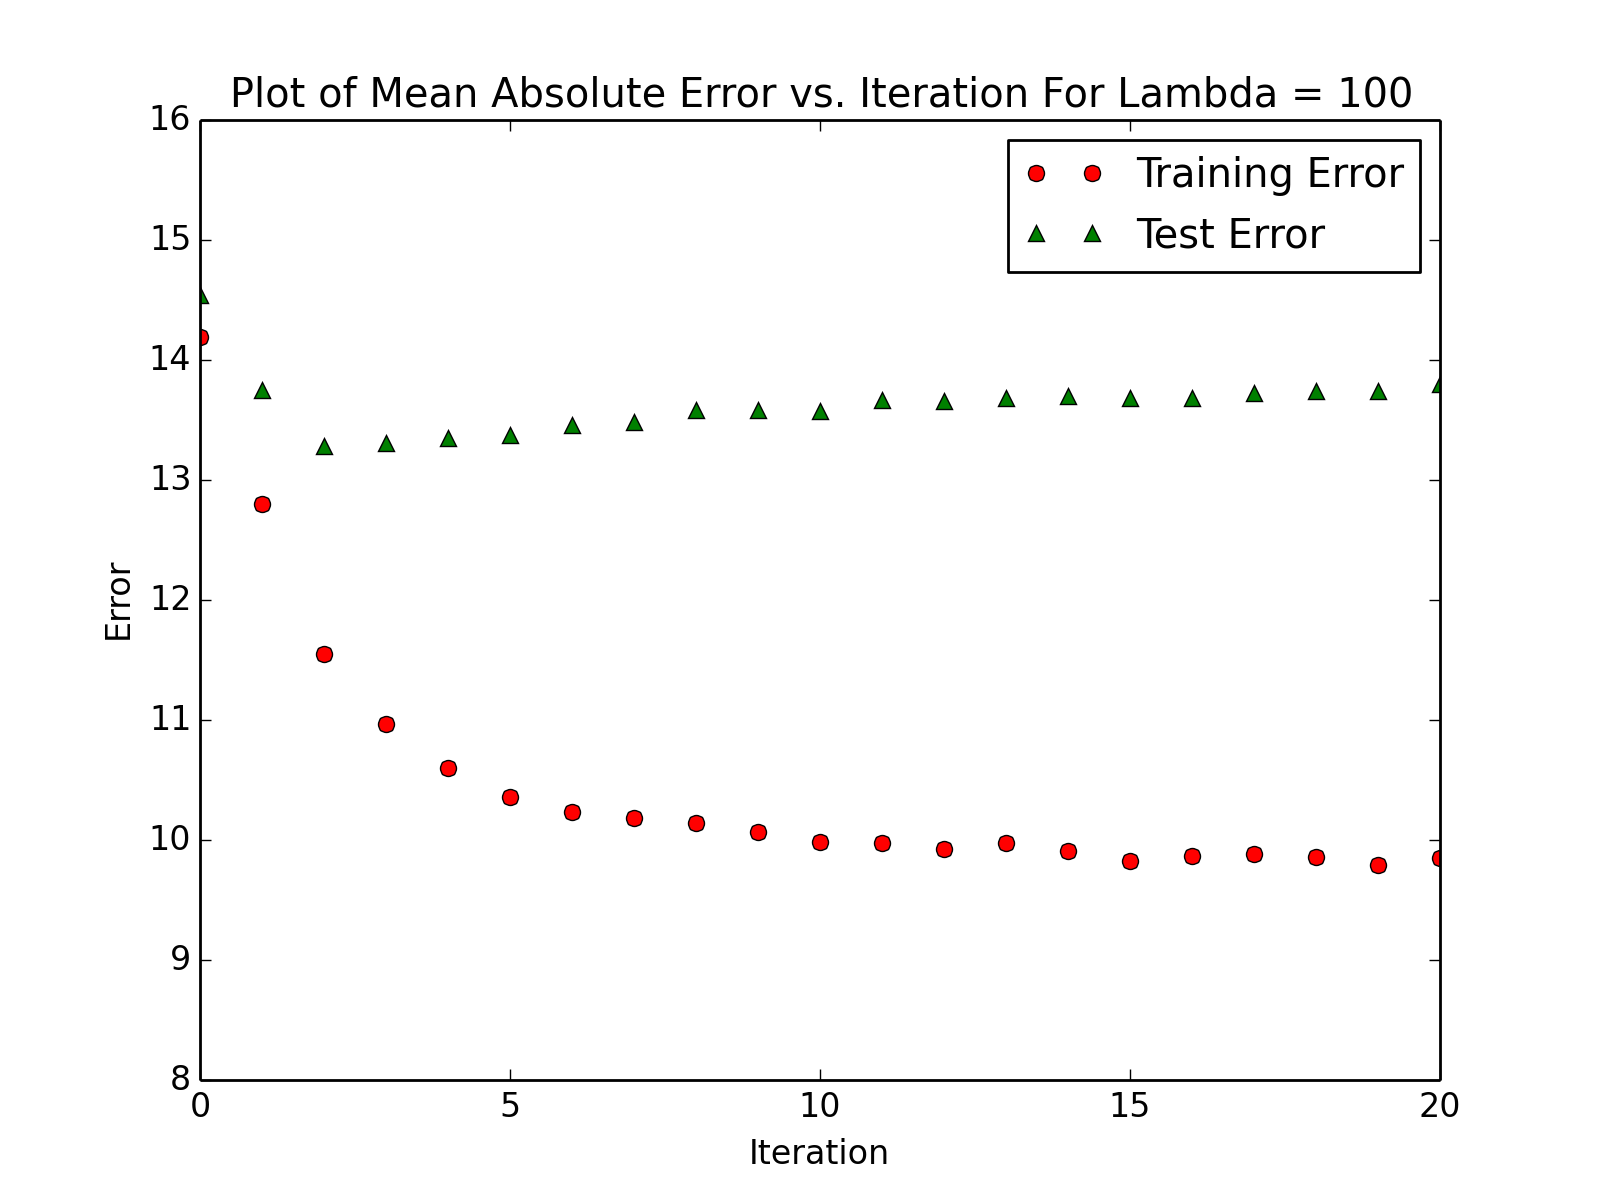
\includegraphics[width=0\factwidth\textwidth,height=\factheight]{matrix_plots/test-i40d25l100.png}
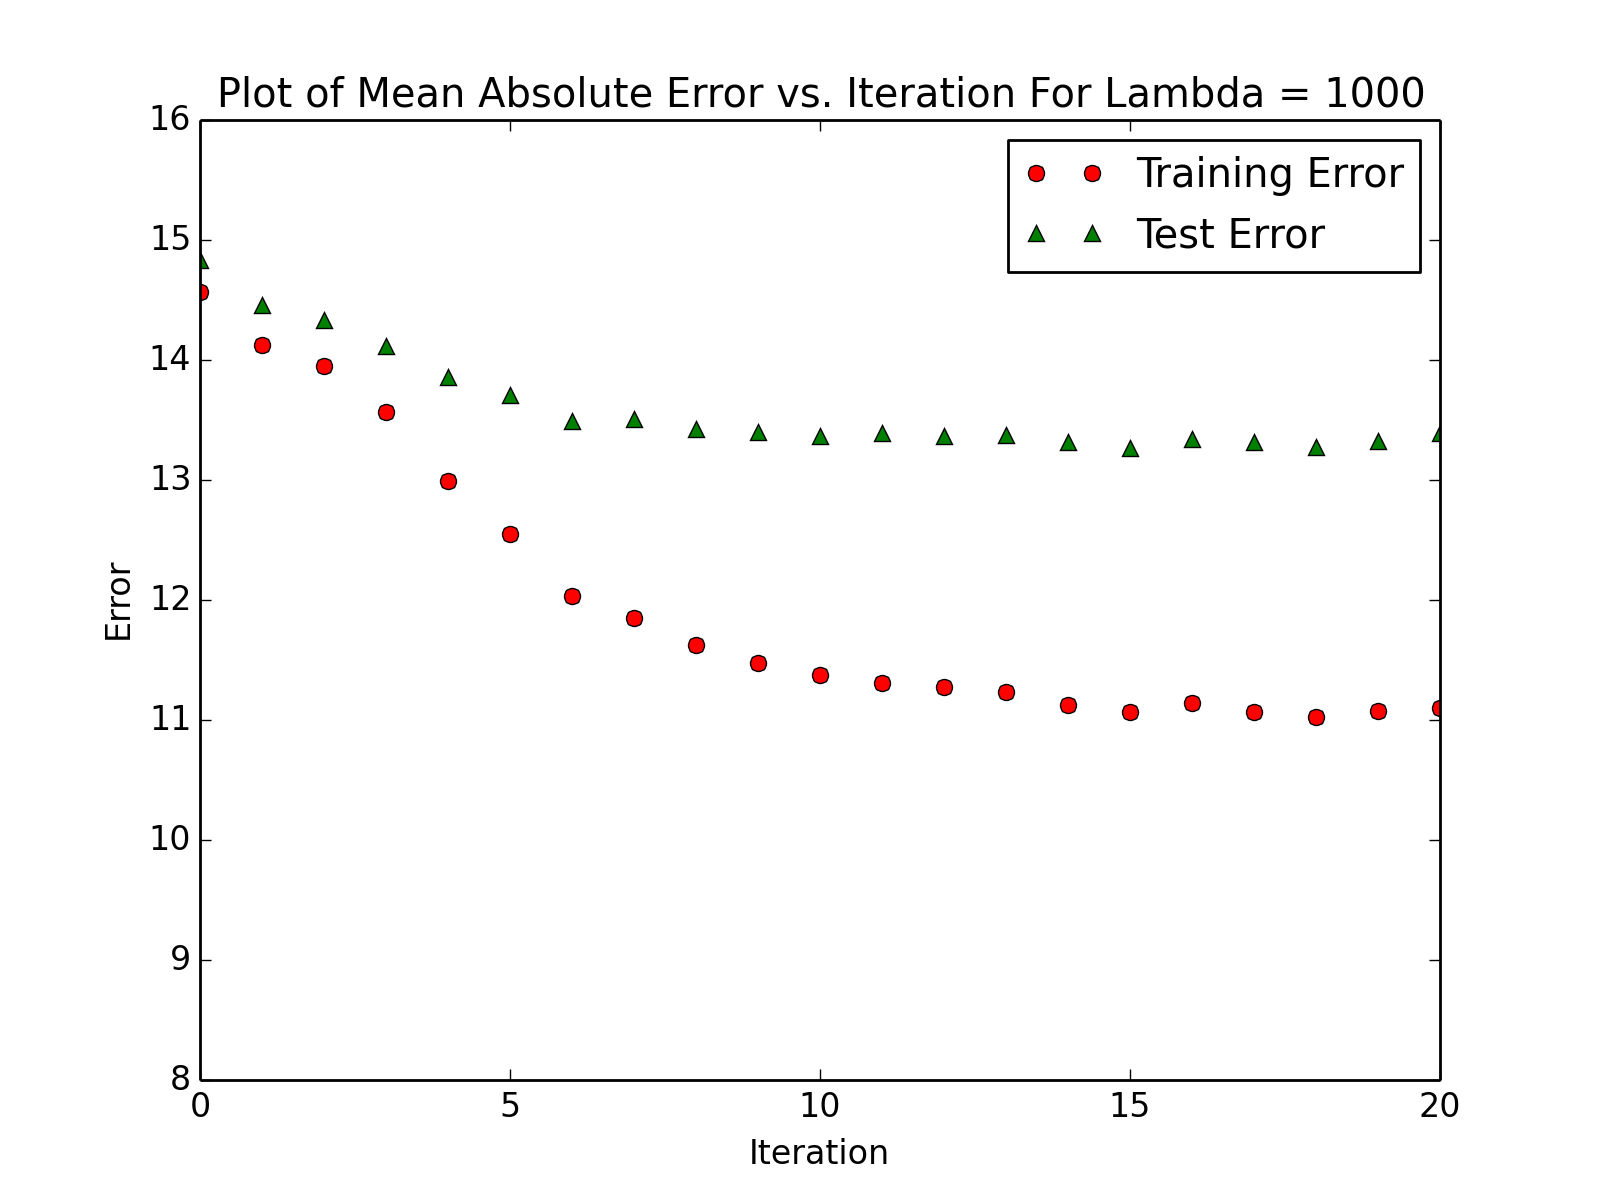
\includegraphics[width=0\factwidth\textwidth,height=\factheight]{matrix_plots/test-i40d25l1000.png}
\caption{Mean absolute training and test error over 20 iterations in the stochastic matrix factorization model. Stocastic gradient descent was performed using a step size of 0.002. The learned critic matrix was count(critics) by 25, and the learned movie matrix was 25 by count(movies).}
\label{fig:fac-d25}
\end{figure}
\begin{figure}[H]
\centering
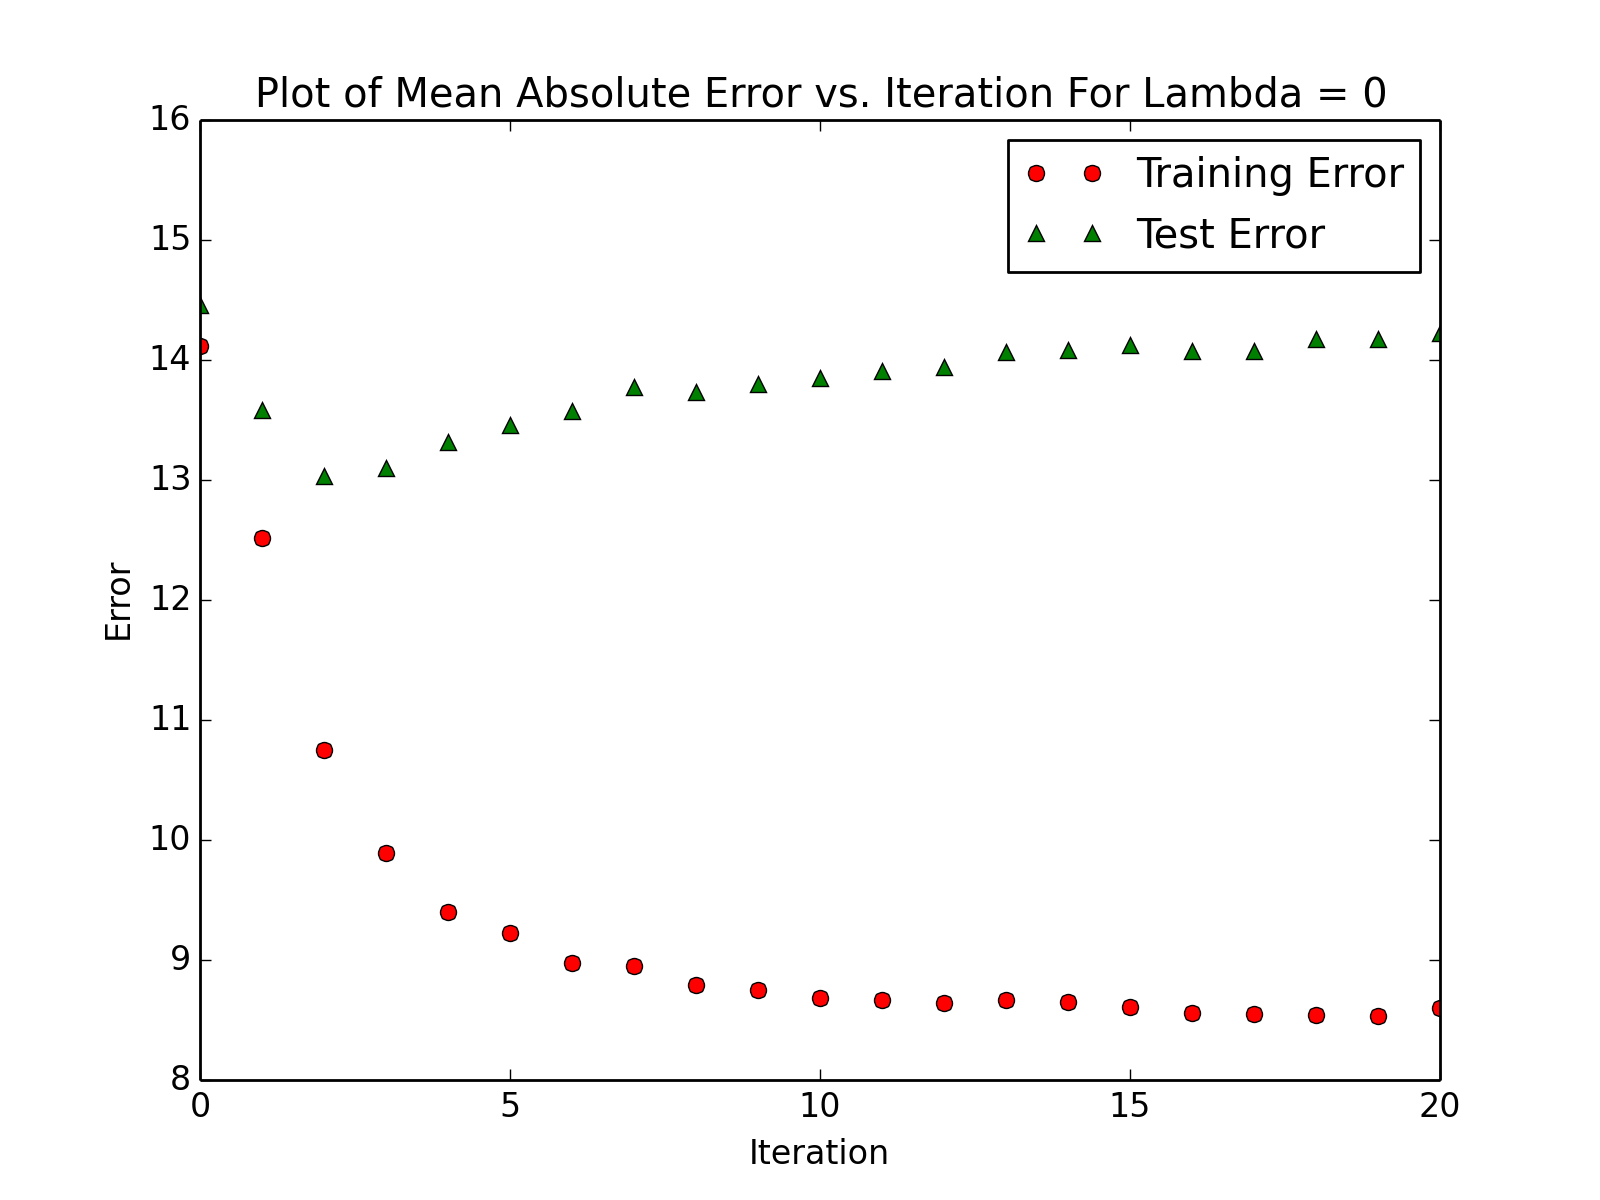
\includegraphics[width=0\factwidth\textwidth,height=\factheight]{matrix_plots/test-i40d40l0.png}
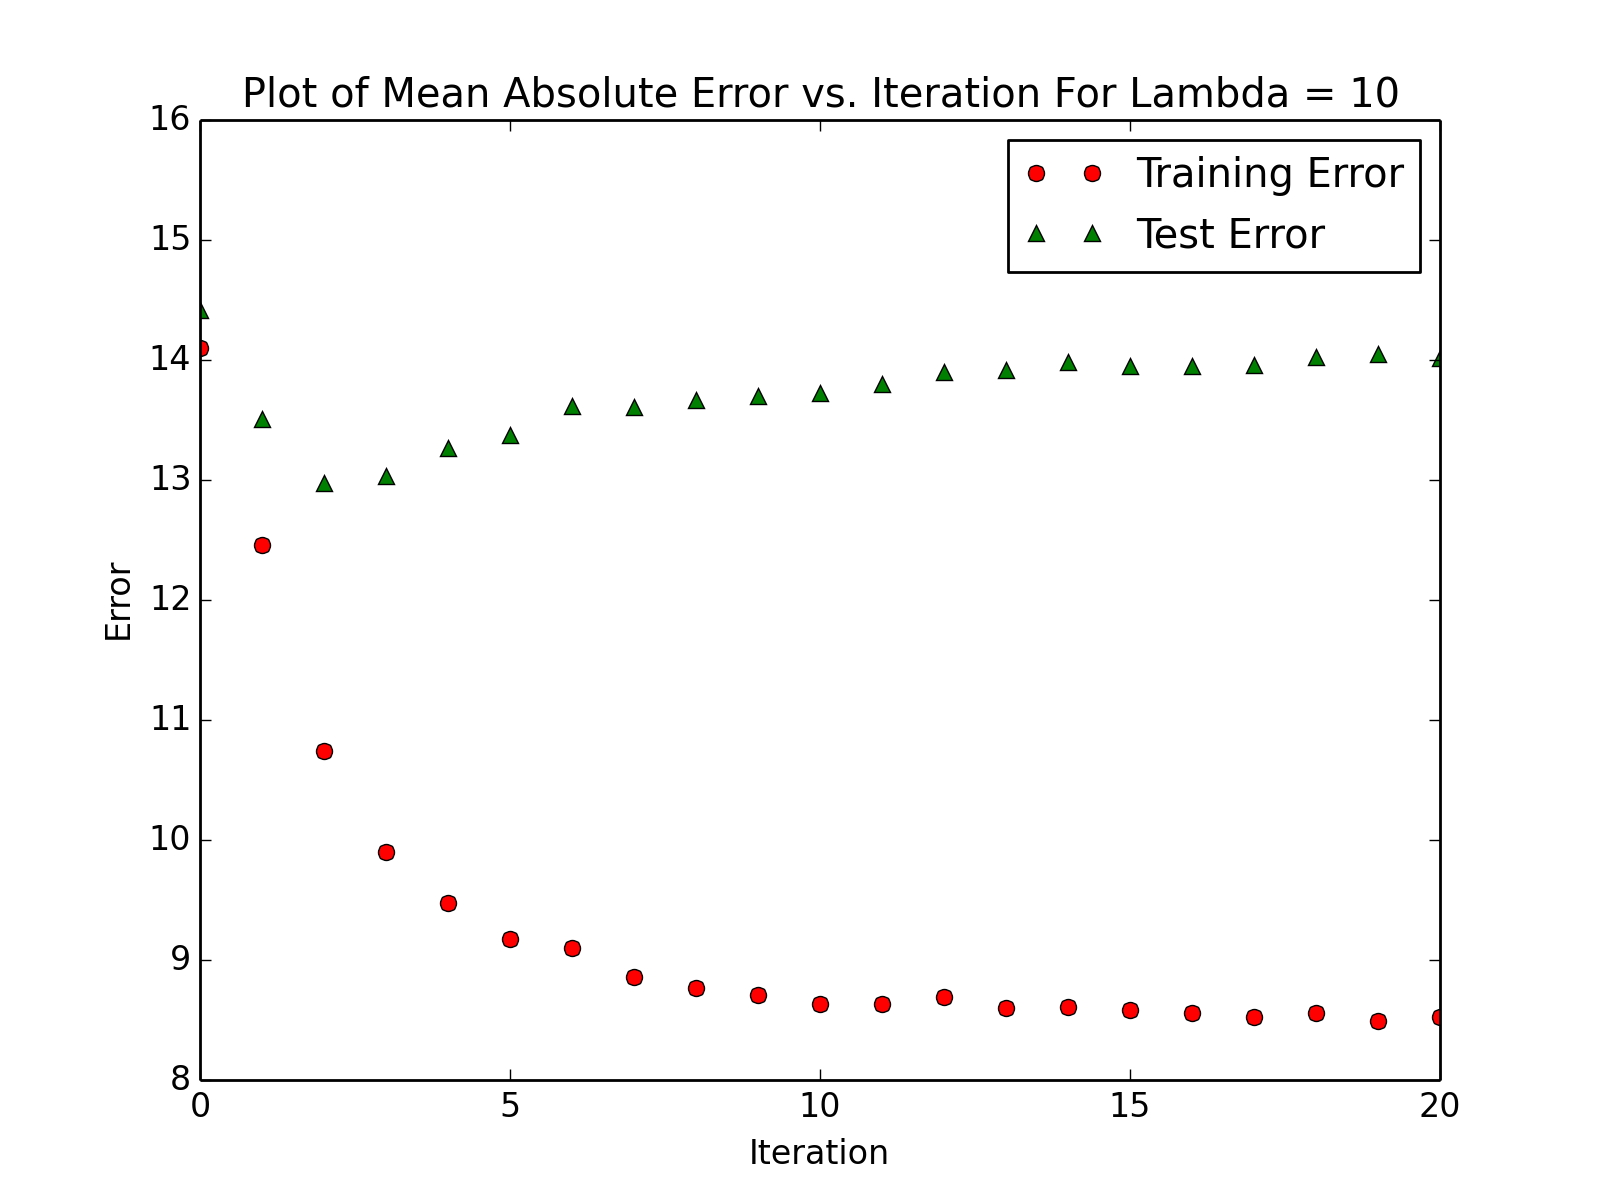
\includegraphics[width=0\factwidth\textwidth,height=\factheight]{matrix_plots/test-i40d40l10.png}
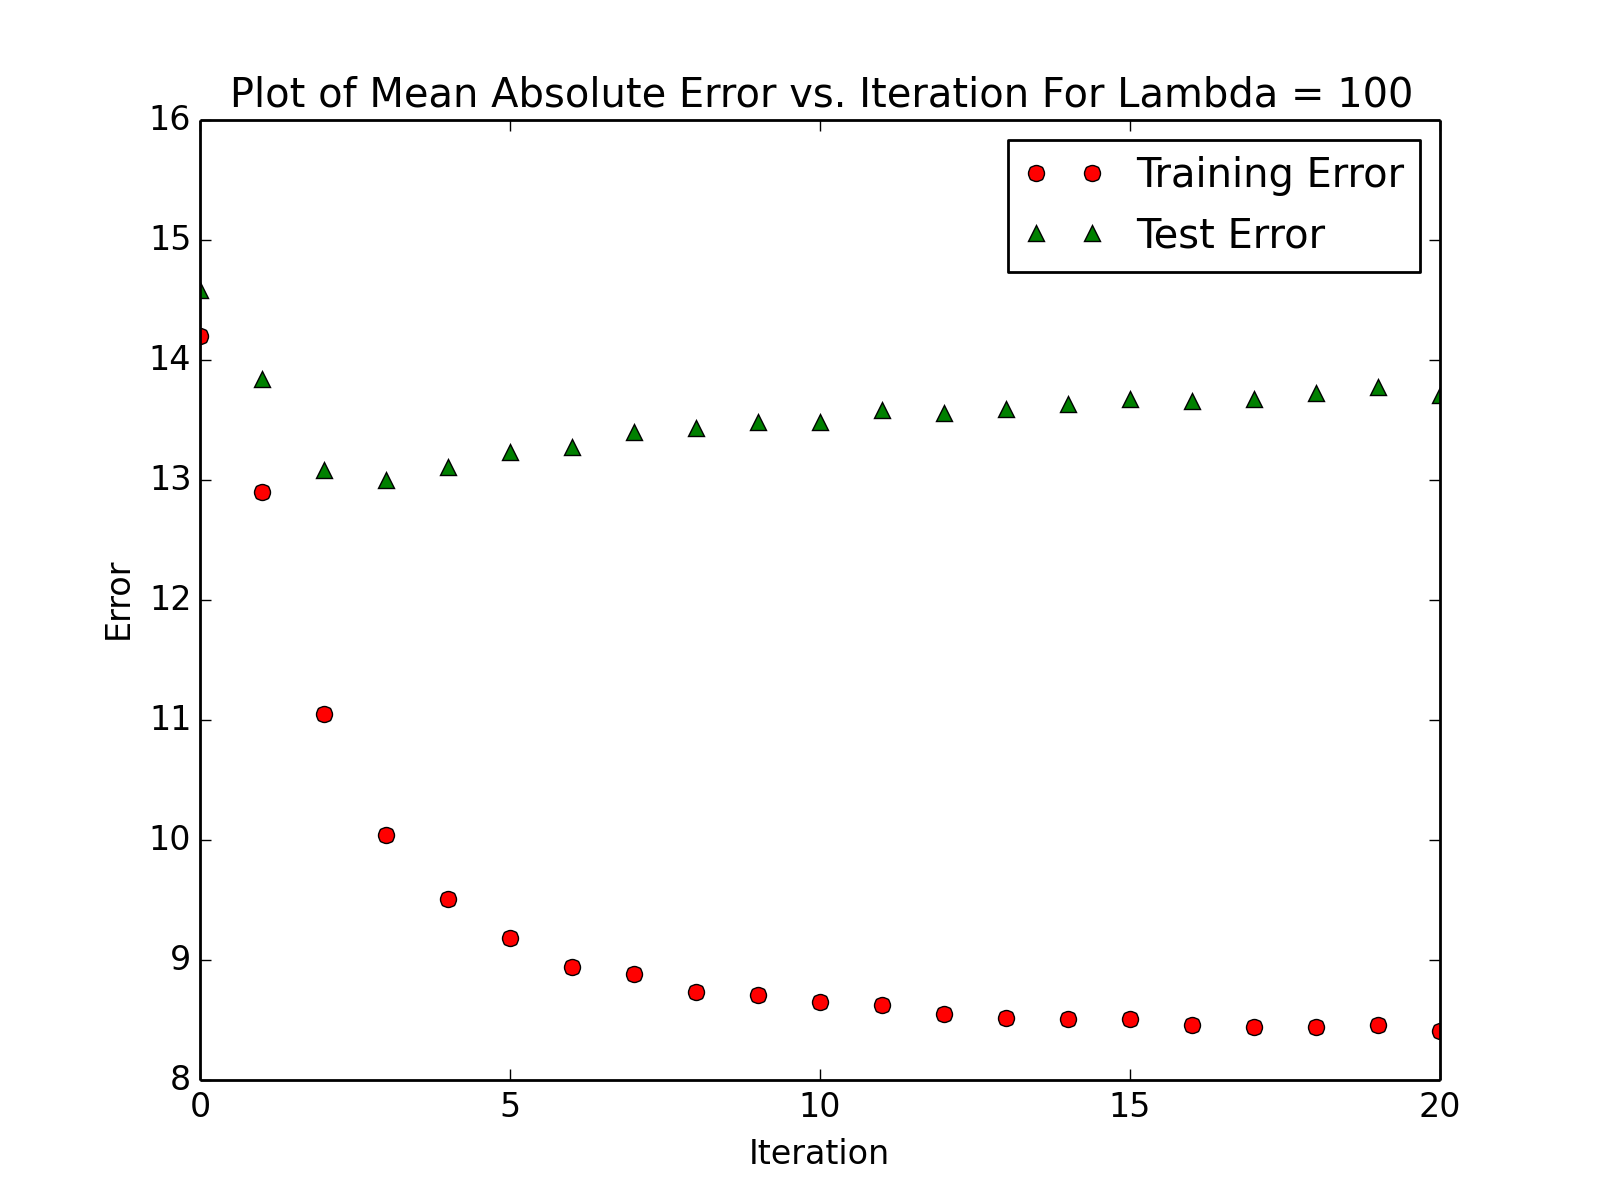
\includegraphics[width=0\factwidth\textwidth,height=\factheight]{matrix_plots/test-i40d40l100.png}
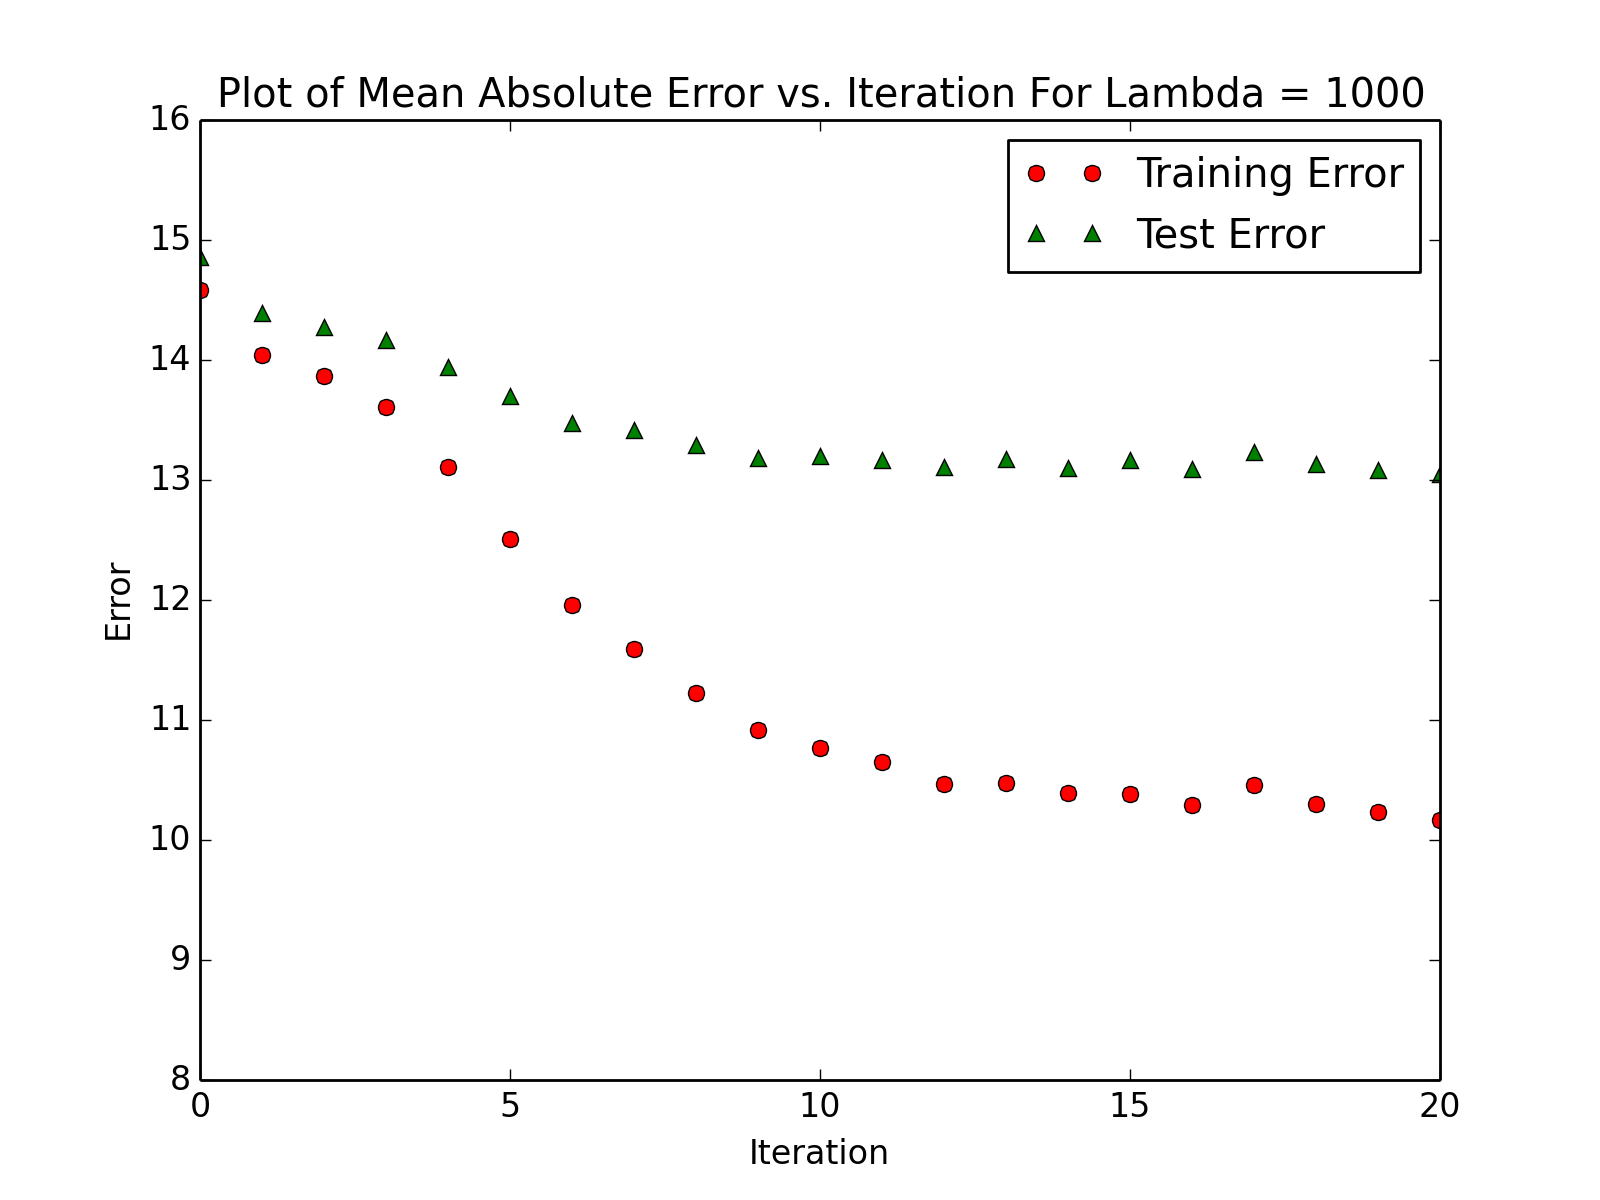
\includegraphics[width=0\factwidth\textwidth,height=\factheight]{matrix_plots/test-i40d40l1000.png}
\caption{Mean absolute training and test error over 20 iterations in the stochastic matrix factorization model. Stocastic gradient descent was performed using a step size of 0.002. The learned critic matrix was count(critics) by 40, and the learned movie matrix was 40 by count(movies).}
\label{fig:fac-d40}
\end{figure}



\section{Collaborative Filtering Results}

To our surprise, even though collaborative filtering appeared to us as a more
natural fit, the results it produced failed to outperform matrix factorization.

Indeed, figure \ref{fig:collab_p}  shows that the collaborative filtering
recommender achieved a mean absolute test
error of 15.5 using adjusted cosine and 14.0 using Pearson correlation, whereas
matrix factorization achieved \matrixtesterror. Of course, the mean error of
rating prediction algorithms is only an indirect measure of the performance of
similarity measures, so it is hard to conclude which approach is better.

Figure \ref{fig:collab_k} shows that the model does not perform significantly
better when estimating ratings using
a weighted average of the 1000 closest critics rather than simply the 10
closest. This points to the fact that few critics are usually close to a given
critic, so only a small number of them will have any significant impact on
the estimated average.

We furthermore observed (see figure \ref{fig:collab_n}) that restricting the
training data to critics having
written a large number of reviews did not have any significant effect on the
mean error. Thus the system can be made more performant by ignoring at least
half of the reviewers.

\begin{figure}[H]
\centering
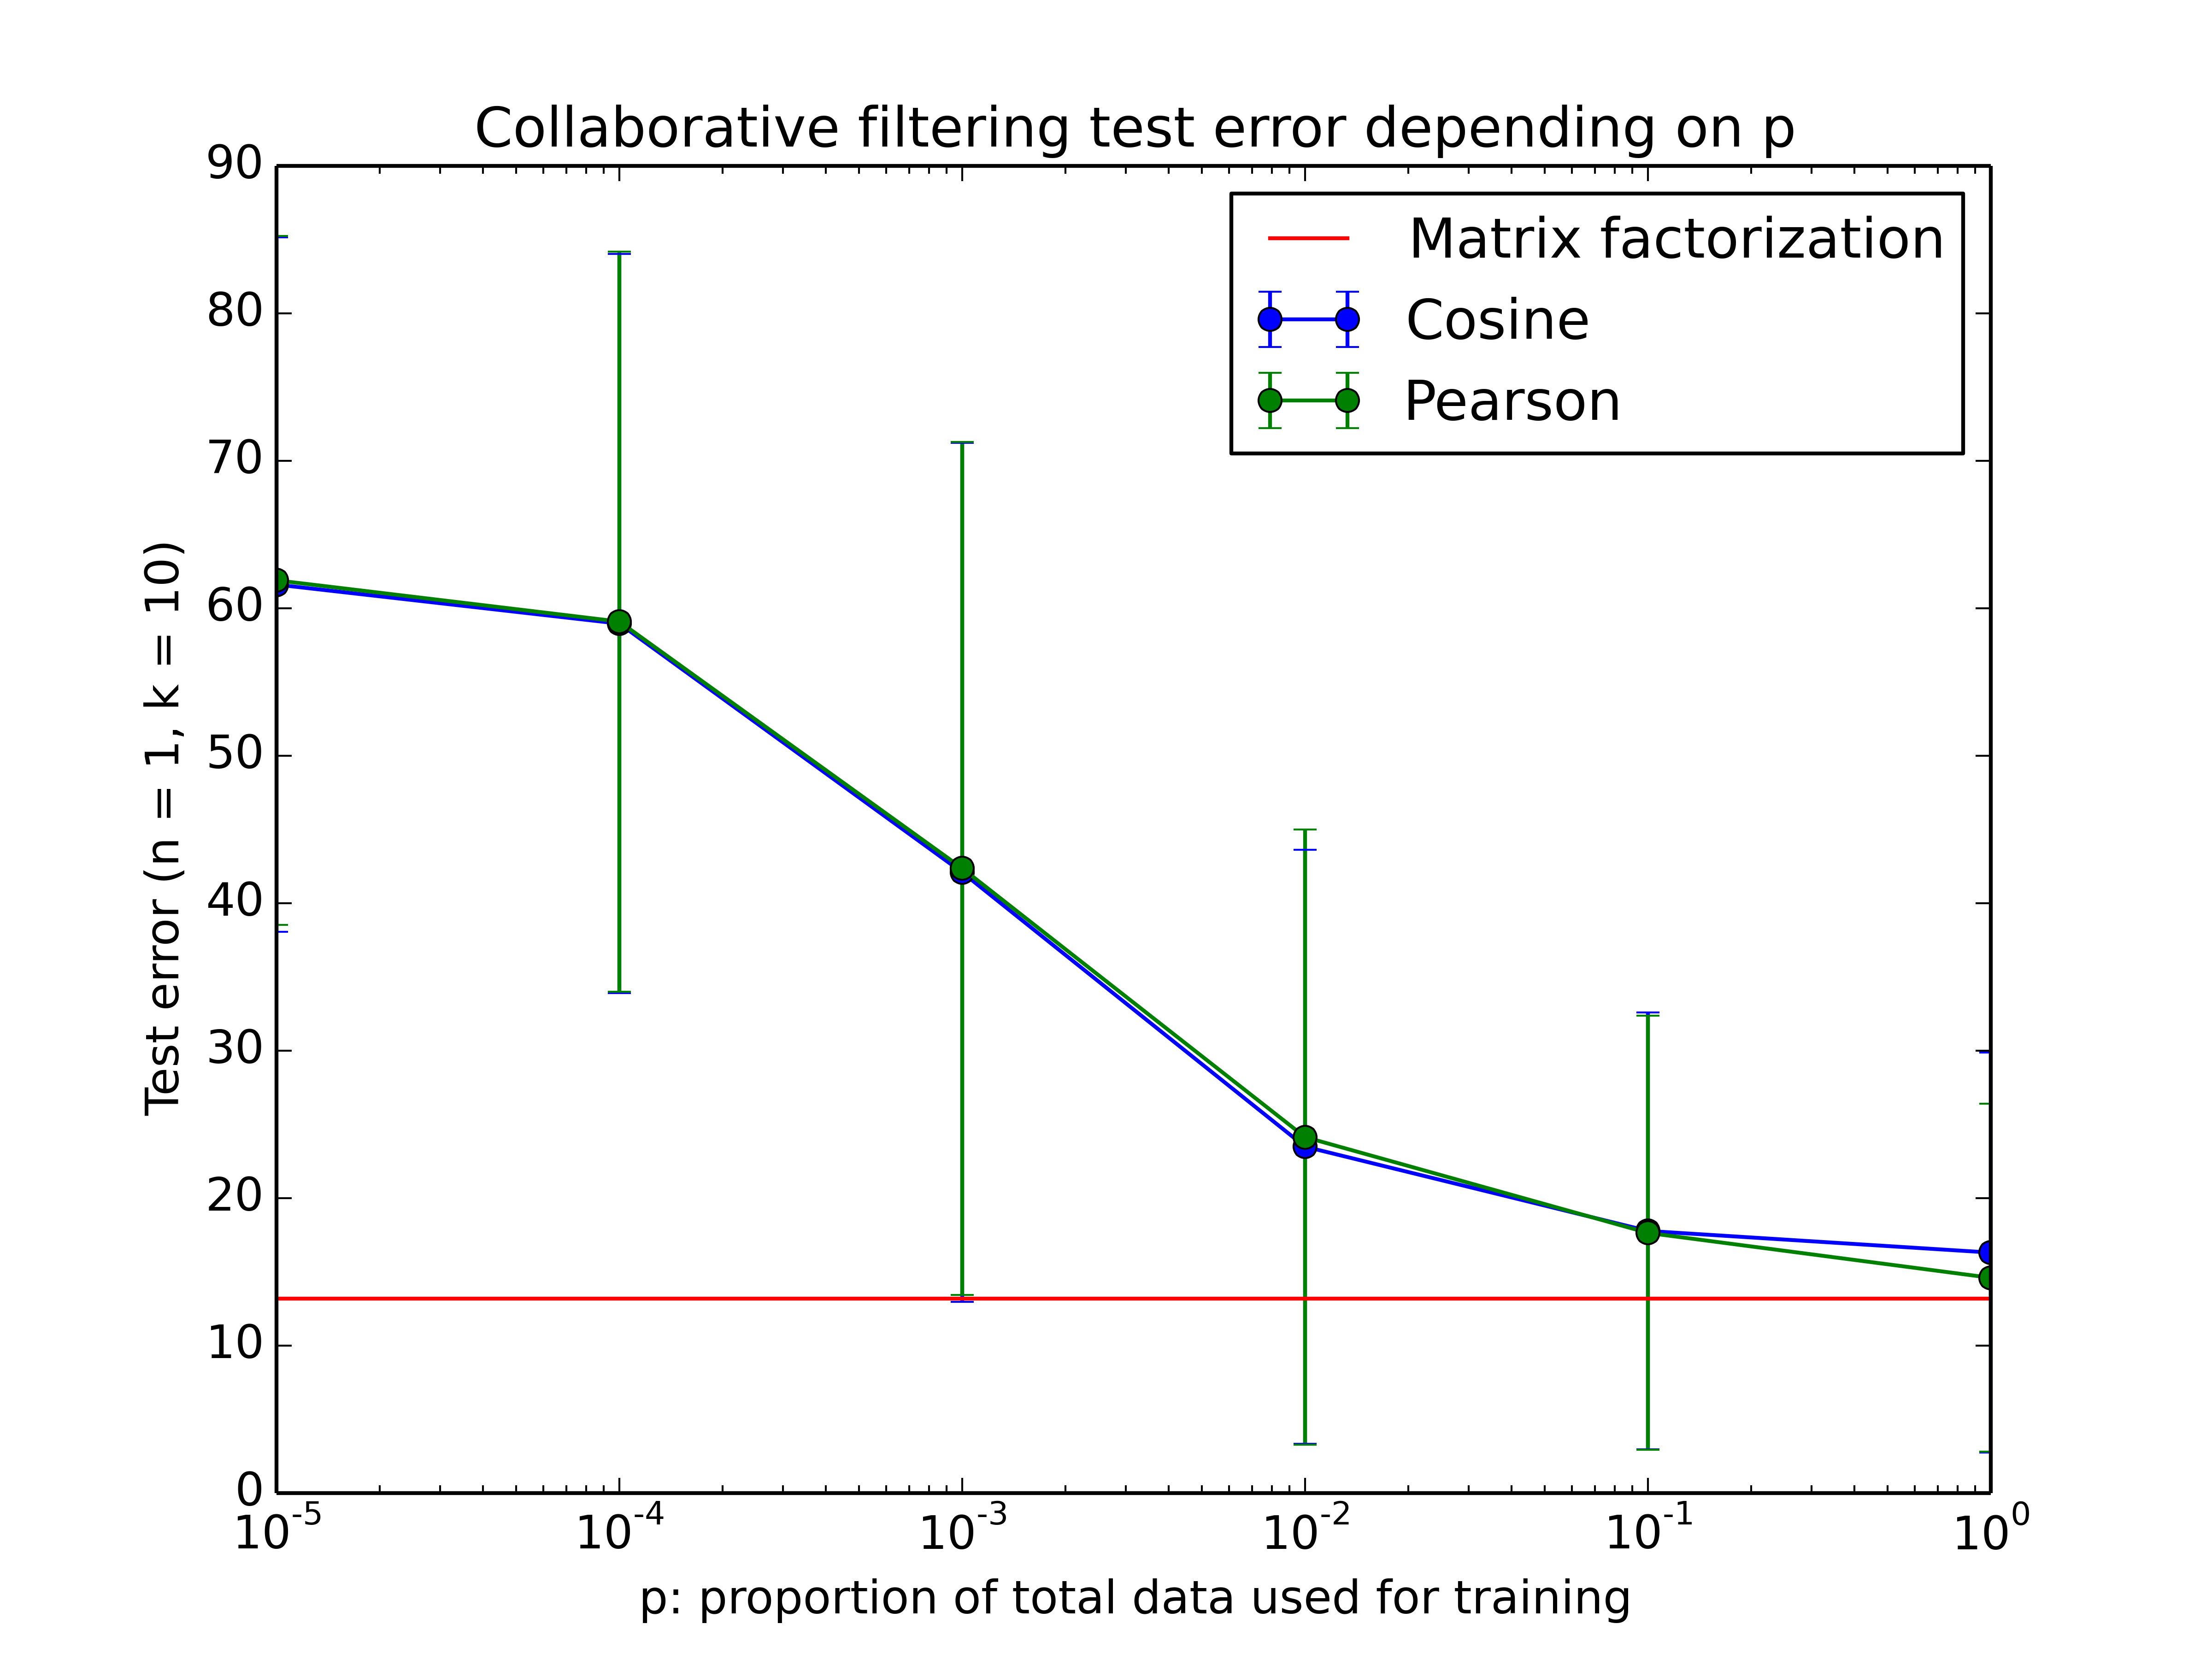
\includegraphics[width=0.7\textwidth]{../plots/collab/graph_p.png}
\caption{Mean test error of the collaborative filtering recommender trained
    over a varying proportion $p$ of the ratings. All critics with at least
    n = 1 review were used for training, and ratings were predicted using the
    k = 10 closest critics.}
\label{fig:collab_p}
\end{figure}

\begin{figure}[H]
\centering
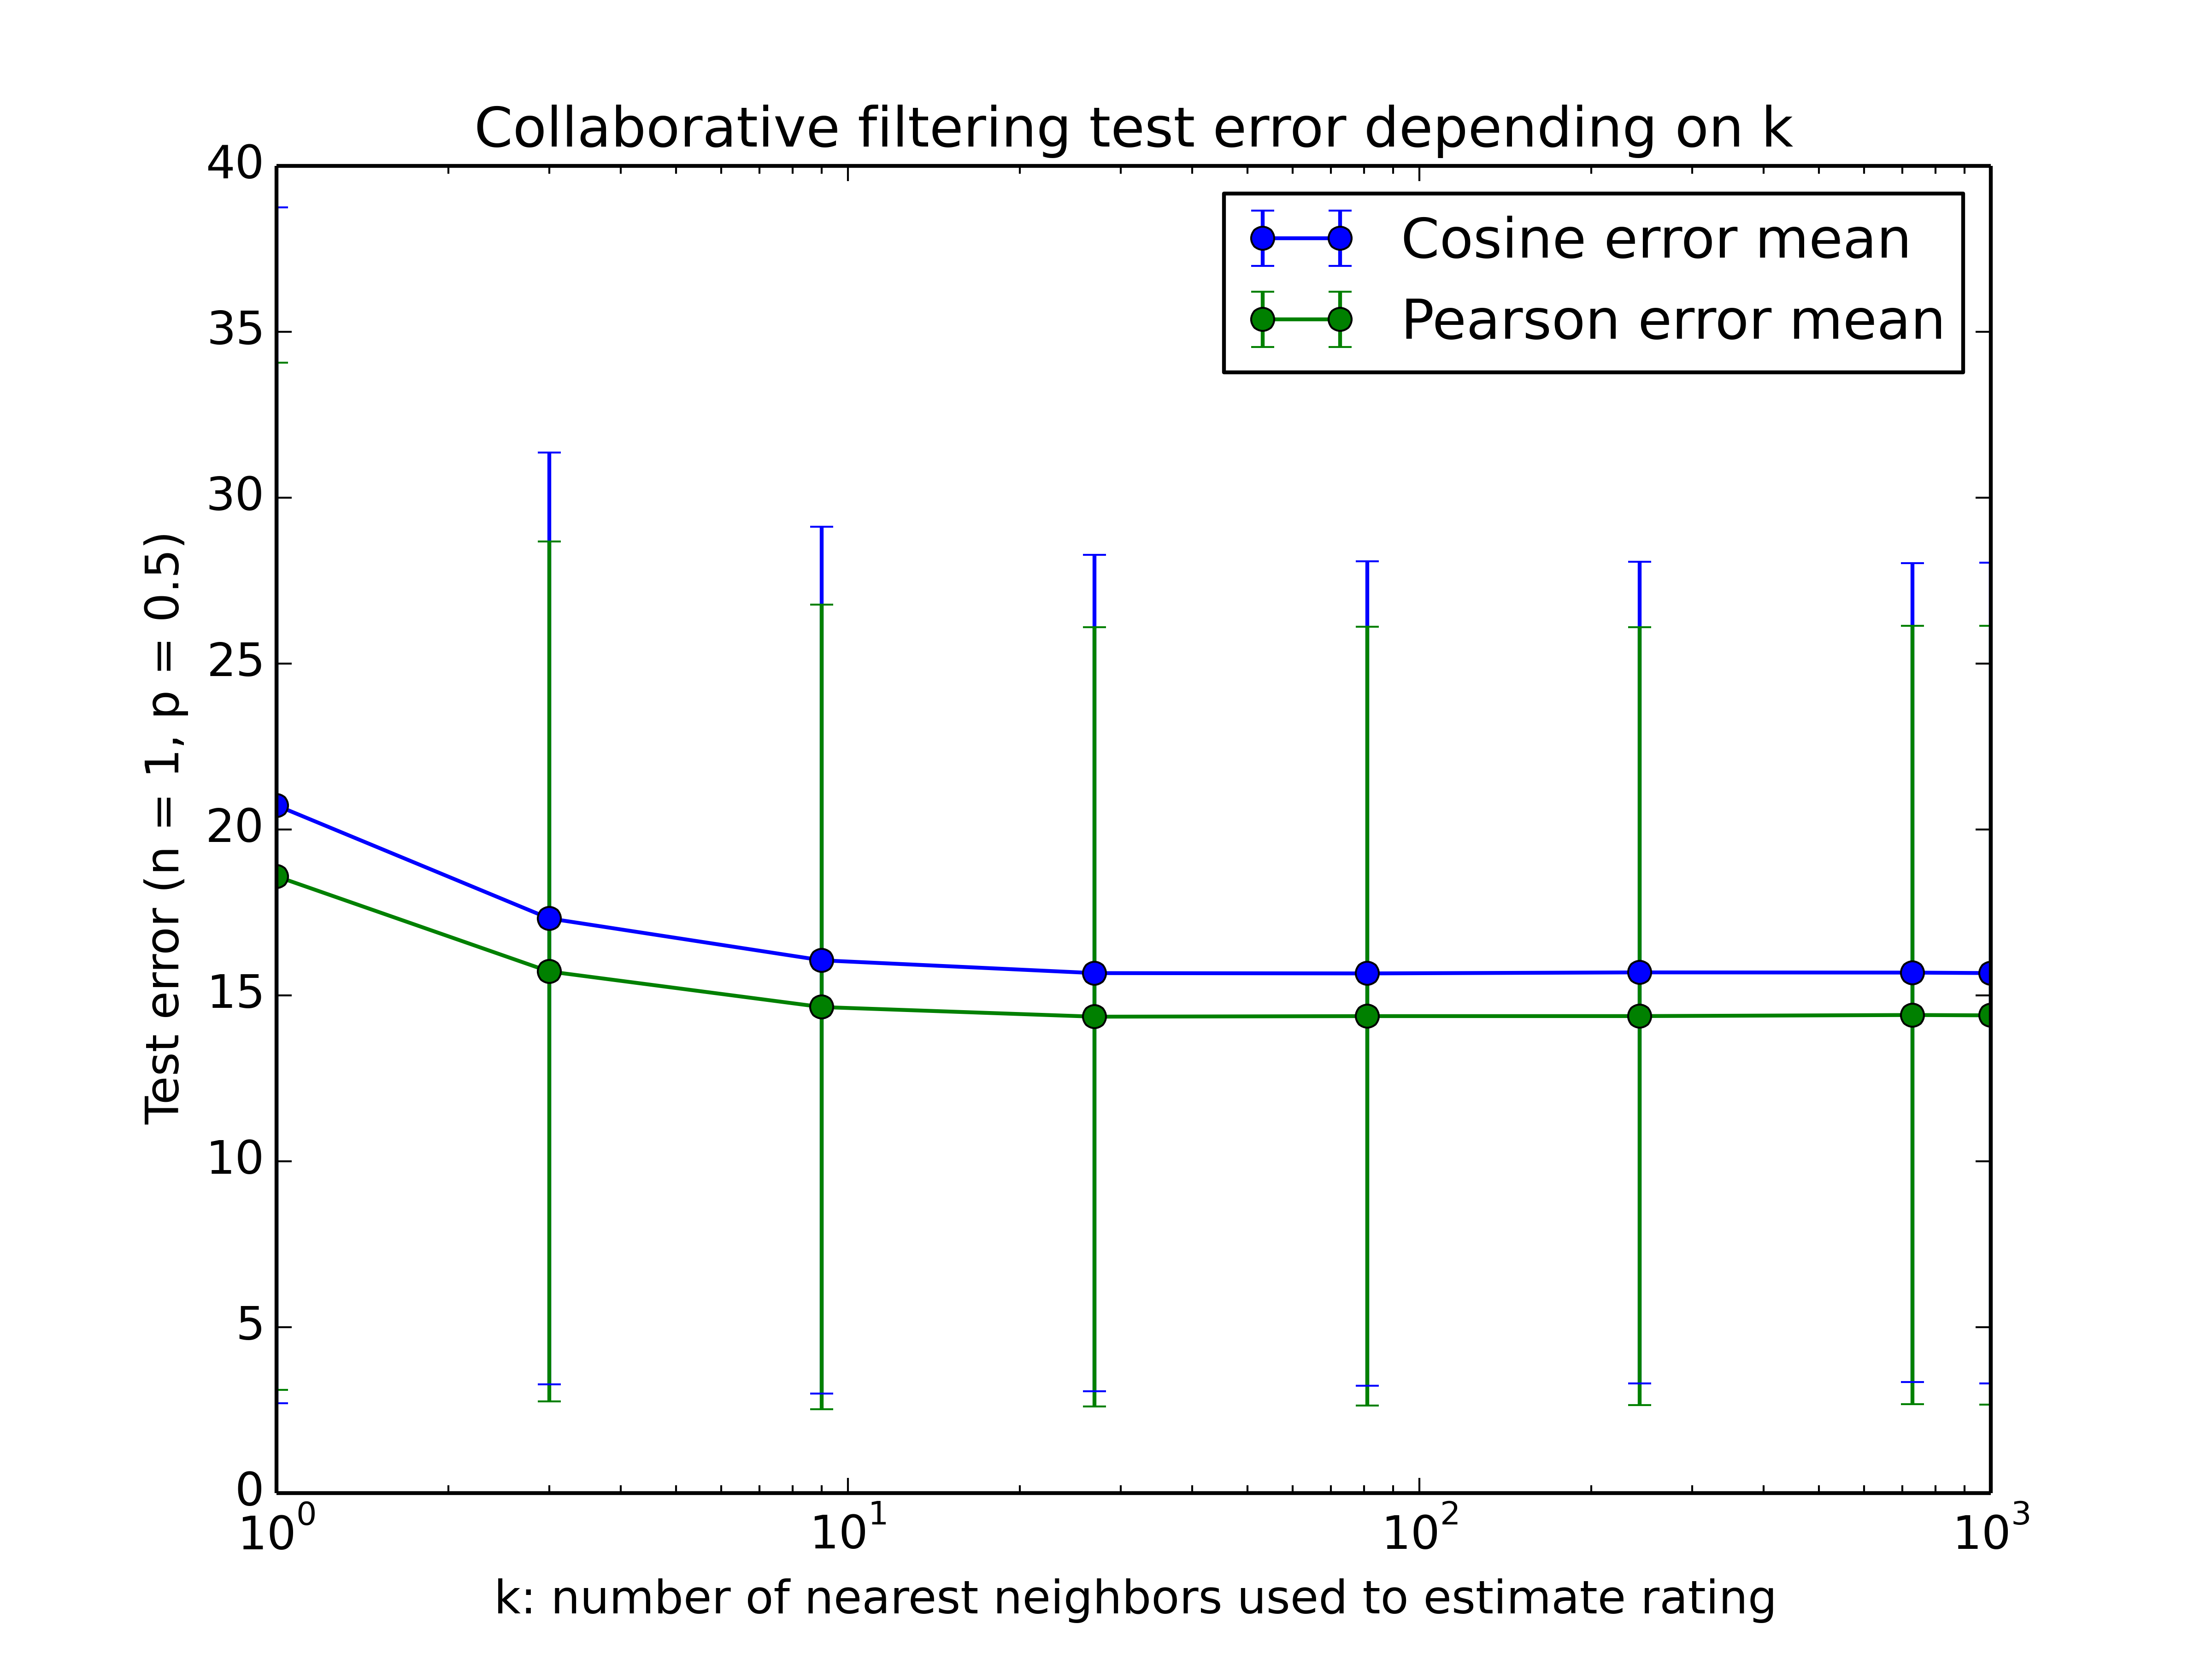
\includegraphics[width=0.7\textwidth]{../plots/collab/graph_k.png}
\caption{Mean test error of the collaborative filtering recommender using a
    varying number k of closest critics. All critics with at least n = 1
    review were used for training, and the model was trained on 50\% of the
    review data.}
\label{fig:collab_k}
\end{figure}

\begin{figure}[H]
\centering
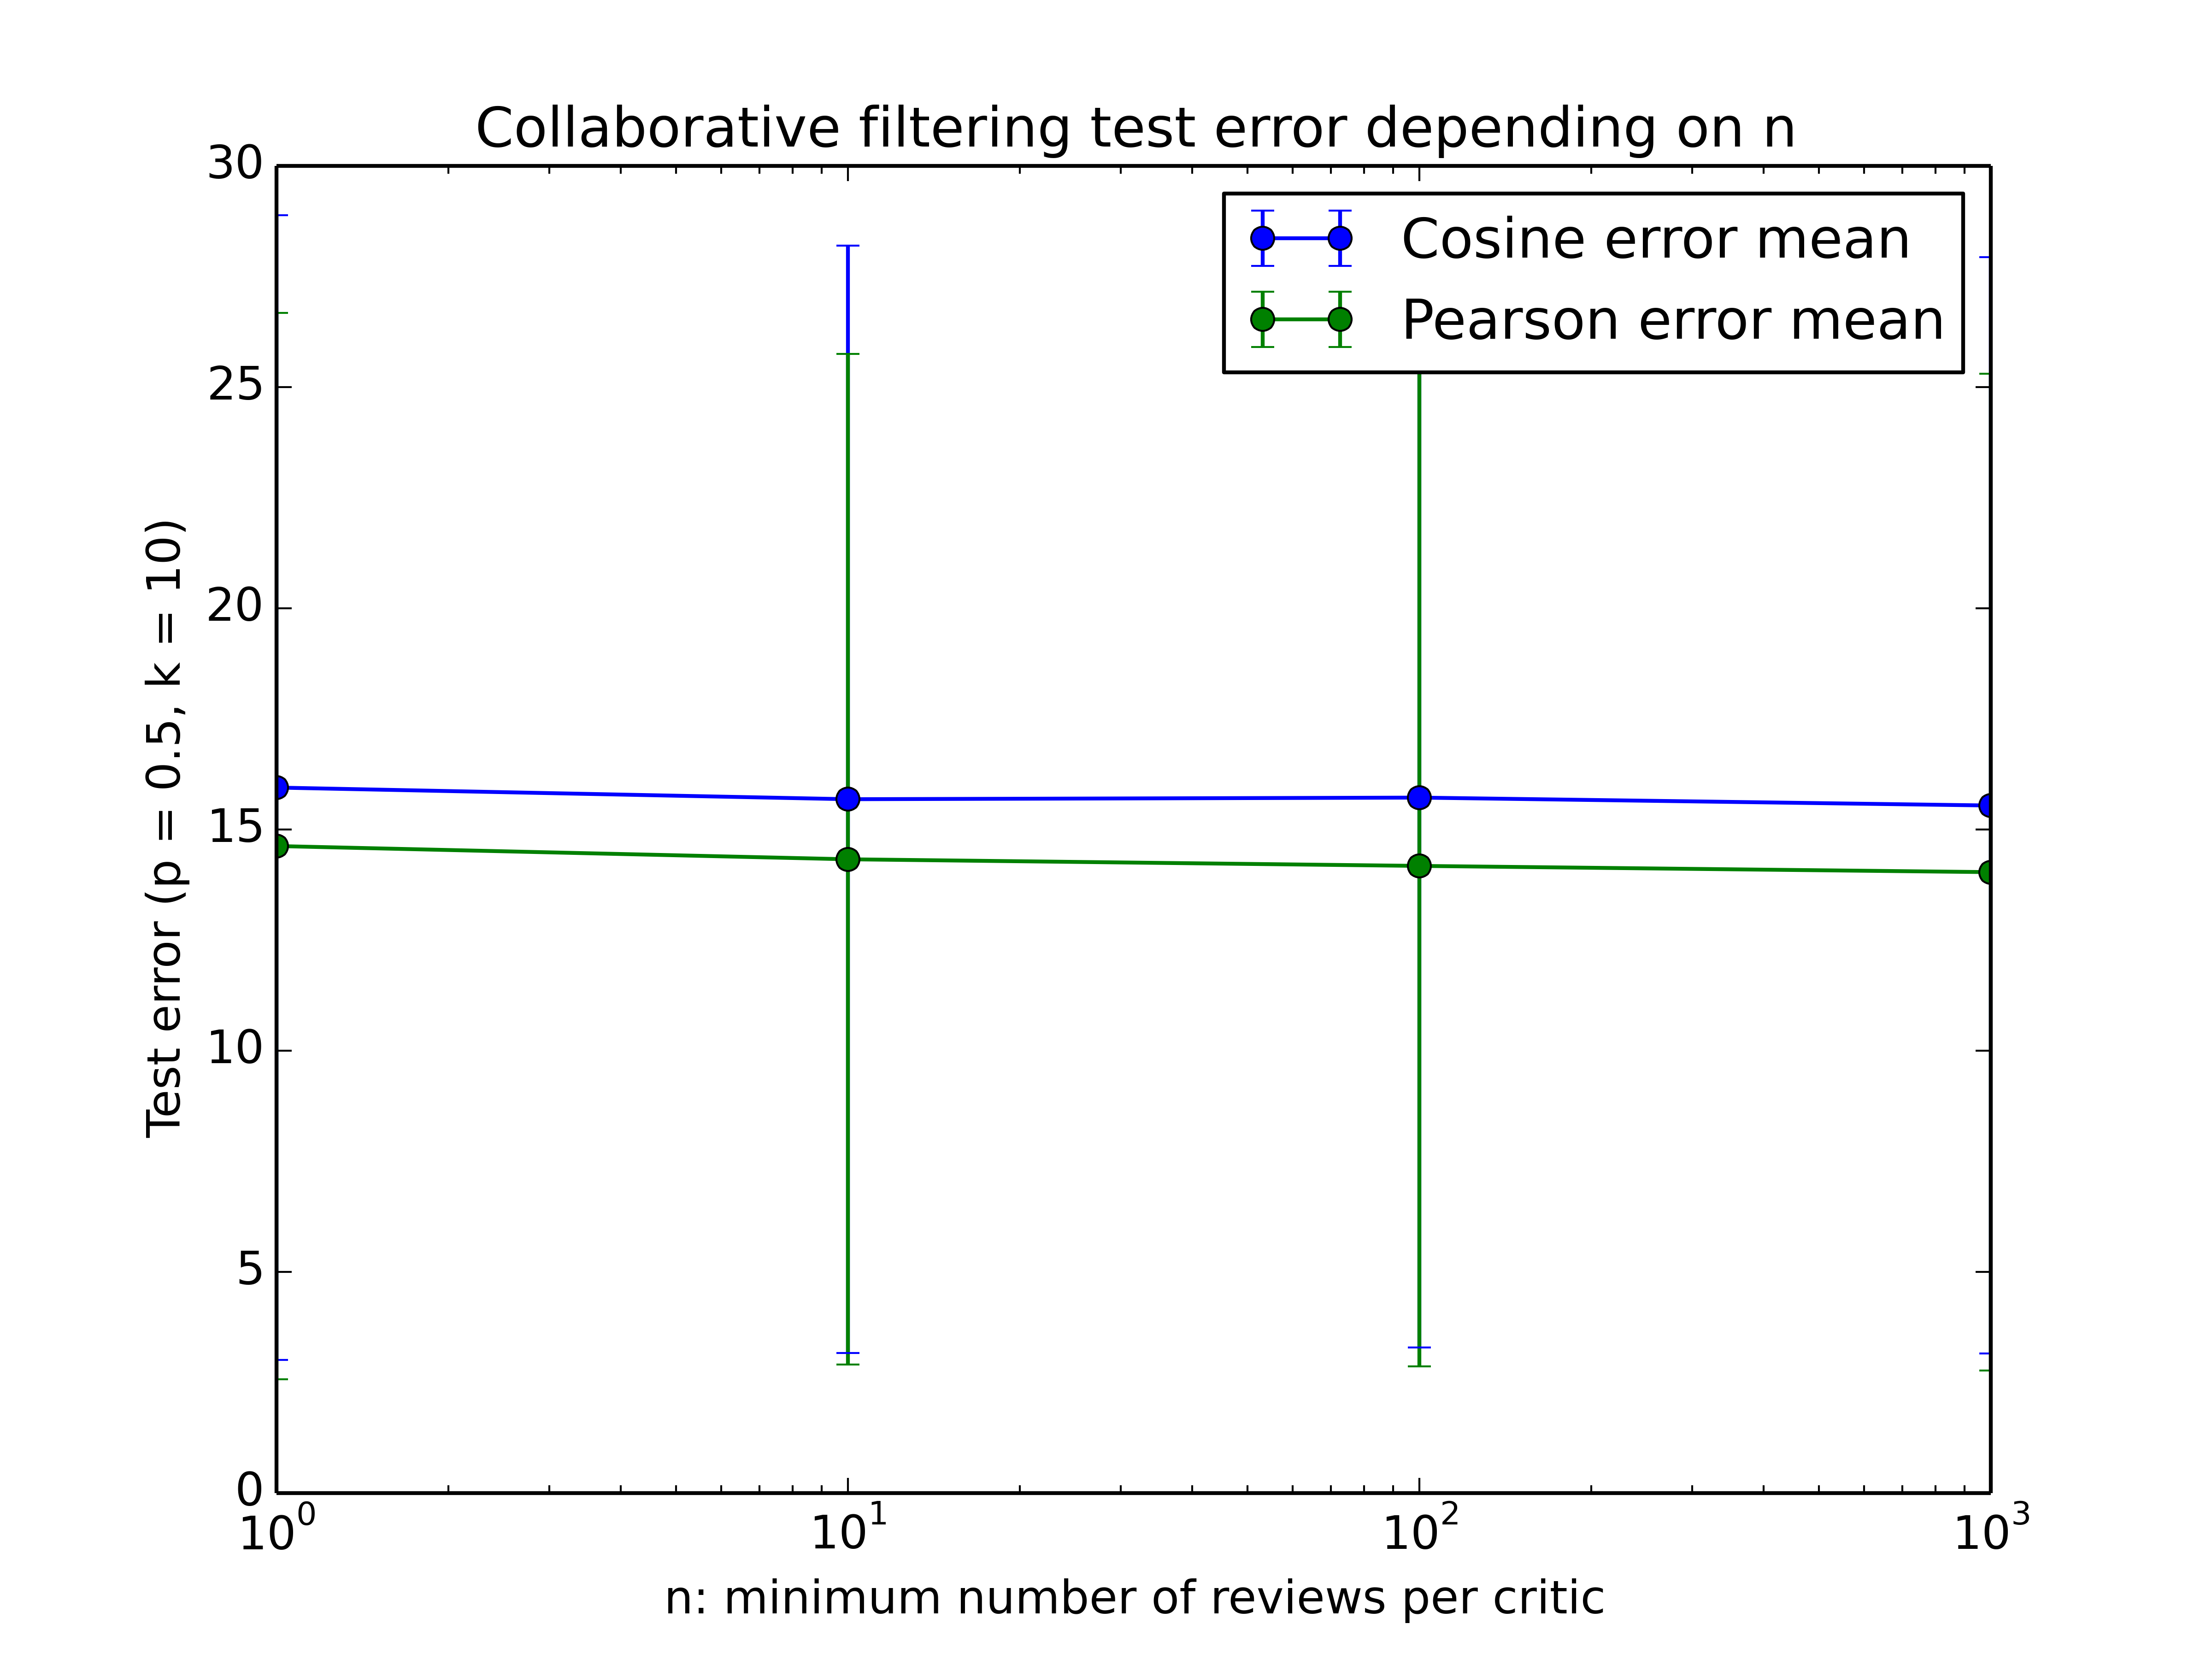
\includegraphics[width=0.7\textwidth]{../plots/collab/graph_n.png}
\caption{Mean test error of the collaborative filtering recommender using only
    those critics having written at least n reviews. The model was trained on
    50\% of the review data, and only the k = 10 closest critics were used to
    estimate ratings.}
\label{fig:collab_n}
\end{figure}

One important difference between matrix factorization and collaborative
filtering lies in the time complexity of both algorithms. Learning the matrix
factorization model is slow ($O(NMi)$ where $N$ is the number of critics, $M$
the number of movies and $i$ the number of iterations), and gets slower with
the number of iterations desired. Once it is done though, similarities between
critics as well as estimated movie ratings can be computed in constant time.

On the other hand, there is no real learning phase in the case collaborative
filtering. One can simply precompute the similarities between critics, which
takes $O(NM)$ time at worst (it can be optimized by using sparse matrix
representations). Then of course computing the similarity between two critics
takes constant time. However estimating a movie rating takes $O(N)$, so
estimating every movie rating for every critic takes $O(N^2M)$, which is
significantly worse than matrix factorization.

In our case, collaborative filtering is significantly faster, as it requires no
learning phase to compute similarities. Estimating ratings may be slower, but
it is only required for performance comparison.

\section{Further work}


The second extension would be to extract more features from data we already have (review publication, movie director, cast, runtime, MPAA rating, etc.) and integrate them in our matrix factorization model. Adding these fixed features to the feature matrices would allow us to more accurately learn the remaining features and therefore enable us to learn a better measure of critic similarity.

The third extension would be to do text analysis on reviews in order to extract critic features (vocabulary, length of reviews, \dots) and movie features (we could learn the movie genre, what emotions it evokes, \dots). This would require a significant amount of work, as sentiment analysis is another entire field of machine learning.

\bibliography{bibliography}{}
\bibliographystyle{plain}

\end{document}
